%-----------------------------------------------------------------------------
%
%               Template for sigplanconf LaTeX Class
%
% Name:         sigplanconf-template.tex
%
% Purpose:      A template for sigplanconf.cls, which is a LaTeX 2e class
%               file for SIGPLAN conference proceedings.
%
% Guide:        Refer to "Author's Guide to the ACM SIGPLAN Class,"
%               sigplanconf-guide.pdf
%
% Author:       Paul C. Anagnostopoulos
%               Windfall Software
%               978 371-2316
%               paul@windfall.com
%
% Created:      15 February 2005
%
%-----------------------------------------------------------------------------


%\documentclass[preprint]{sigplanconf} 

% The following \documentclass options may be useful:
%
% 10pt          To set in 10-point type instead of 9-point.
% 11pt          To set in 11-point type instead of 9-point.
% authoryear    To obtain author/year citation style instead of numeric.

%\usepackage{amsmath}
%\usepackage{graphicx}
%\usepackage{placeins}
%\usepackage{tikz}
%\usepackage{pgfplots}
%\usetikzlibrary{shapes,snakes,positioning}
%\usepackage{fancyvrb}
%\usepackage[T1]{fontenc}
%\newcounter{arraycard}

%\begin{document}

%\conferenceinfo{WXYZ '05}{date, City.} 
%\copyrightyear{2005} 
%\copyrightdata{[to be supplied]} 

%\titlebanner{DRAFT}        % These are ignored unless
%\preprintfooter{Obsidian: GPU kernel generation}   % 'preprint' option specified.

%\title{Embedded Language for High Performance GPU Computing}
%\title{Towards An Embedded Language\\ for High Performance GPU Computing}  
%\title{An Embedded Language for Resource Aware \\ GPU Kernel Programming}  
%\title{A High-Level Embedded Language for Low-Level GPU Kernel Programming}  

%\subtitle{Subtitle Text, if any}

%\authorinfo{Bo Joel Svensson \and Mary Sheeran} 
%           {Chalmers University of Technology}
%           {\{joels,ms\} at chalmers dot se} 

\newcommand{\subsubsubsection}[1]{\paragraph{#1:}}
%% \vspace{1ex}

%% \noindent\emph{\bf#1}\newline

%% \vspace{1ex}
%% \noindent
%% } 


%\maketitle
% ---------------------------------------------------------------------------
%
% --------------------------------------------------------------------------- 
\subsection*{abstract}
%\begin{abstract}

Graphics Processing Units (GPUs) offer potential for very high performance;
they are also rapidly evolving. Obsidian is an embedded language (in Haskell) 
for implementing high performance kernels to be run on GPUs. We would like to 
have our cake and eat it too; we want to raise the level of abstraction at 
which the programmer works from that of CUDA code (which we generate) and 
still to give the programmer fine control over low level details.

We present the user's view of Obsidian by showing case studies and a 
detailed optimisation effort applied to reduction kernels. Our chosen array 
representations (pull and push arrays) provide fine control over the use of 
memory, but are also sufficiently abstract to give guaranteed fusion of composed 
array operations. The case studies also show that Obsidian helps to make 
exploration of the design space for kernels easy. Code reuse 
and composition is easier in Obsidian than in CUDA. 

Obsidian uses types to model the hierarchical nature of the GPU, to help 
the programmer to write suitable (and easy to compile) GPU programs. Type 
directed compilation provides the user with language constructs that can be 
used at different levels of the GPU hierarchy; the types constrain the allowed 
behaviour of programs at different levels, while remaining reasonably unobtrusive.
The way in which the hierarchical structure of the GPU architecture
has influenced the design of Obsidian is a major theme of this paper.
Thus, the paper may function as an introduction to GPUs and GPU programming 
for functional programmers.

%We illustrate this by showing details of some kernel optimisations; we make use of two different array representations, which we call pull and push arrays. Obsidian also uses types to model the hierarchical nature of the GPU, to help the programmer to write suitable (and easy to compile) GPU programs. Benchmarks show that the low-level, detailed control offered to the programmer does have an associated pay-off in running time.


%Obsidian is an embedded language for 
%implementing high performance GPU kernels while raising the abstraction 
%level, yet maintaining low-level control. We illustrate this by showing 
%case studies and a detailed optimisation effort applied to reduction kernels. 

%Obsidian uses types to model the hierarchical nature of a GPU, both 
%to help the programmer write suitable GPU programs and to allow the 
%implementation of hierarchy agnostic functions. 

% We also present a simple and direct method of monad reification. 

Benchmarks show that the low-level, detailed control offered to the 
programmer does have an associated pay-off in running time. 



%This paper is tutorial in nature and gives much detail about the choices 
%we made in relation to GPU architectures. 

%\end{abstract}

%\category{CR-number}{subcategory}{third-level}
%\category{D.3.2}{Programming Languages}{Language Classifications}[Applicative (functional) languages; Concurrent, distributed, and parallel languages]
%\category{D.3.4}{Programming Languages}{Processors}[Code generation]

%\terms
%term1, term2
%\terms
%Languages, Performance

%\keywords
%keyword1, keyword2
%\keywords
%Data parallelism, array programming, embedded language

% ---------------------------------------------------------------------------
% INTRODUCTION 
% --------------------------------------------------------------------------- 
\subsection{Introduction}

Graphics Processing Units (GPUs) offer potential for high 
performance implementations of data parallel computations. However, 
GPUs are a bit quirky to program; often, the programmer needs to consider 
very low-level concepts in order to make the best use of the GPU. 
GPU programming models mirror the hierarchy of the GPU, with threads, groups of
threads with special properties and then groups of such groups.
There is a matching memory hierarchy, ranging 
from slow global memory that is accessible to all
threads to fast local memory that allows threads within a single
group of threads to communicate with each other.
For NVIDIA GPUs, both the architecture and the programming model are called
CUDA (for Compute Unified Device Architecture). GPU \emph{kernels} are compiled
to run
on the GPU, while serial {\em host code} controls
how they are launched and supplied with data. Here, the word 
kernel denotes an SPMD (Single Program Multiple Data) program that is 
run on the GPU. Section \ref{sec:GPU} covers GPU architecture. 


Obsidian is an embedded language for GPU programming that aims to raise the 
level of abstraction for the GPU programmer, while maintaining control over 
the low-level details that are needed for performance. 
So far,
we have chosen not to try to apply automatic transformations or compiler 
optimisation techniques to a GPU architecture agnostic program and hope 
to get performance. In Obsidian, we want to put the tools to make the 
correct decisions into the hands of the programmer. From Obsidian programs, 
CUDA kernels are generated, while host code must still be written in CUDA.
For key building blocks like scan and reduce, we see a trend towards
the use of fewer and much more complicated kernels~\citehl{merrill}, so
that the host code is often relatively simple. We wish to support the construction of these sophisticated kernels.


% ---------------------------------------------------------------------------
% Motivation and Contributions
% --------------------------------------------------------------------------- 
\subsubsection{Motivation and contributions} 

Obsidian aims to provide a higher-level language with a more concise programming style than that of CUDA. We want to achieve 
this while keeping programmer control over the details that influence 
performance. The programmer should be able to experiment with global memory 
access patterns, make tradeoffs between sequential computation per thread 
and parallel computations across threads (using shared memory) and avoid 
unnecessary synchronisation. 
%to synchronise unnecessarily. 
%We illustrate these contributions in the 
%case studies and benchmarks section. (section \ref{sec:CASESTUDIES}). 

We envision the user of Obsidian as someone who is familiar with and 
interested in the details of GPU hardware. For this category of users,
the value of Obsidian can be in the rapid prototyping of programming ideas.
Obsidian is also useful for trying to understand the actual cost model
of a particular GPU, since it is so easy to generate programs that are
systematically varied.

Another possible use of Obsidian could be as the code generating backend of 
a domain specific language that could 
benefit from GPU acceleration. Reference ~\citehl{BEAUTY} is an example of this.   
%One such experiment can be found in 
%

Our work on Obsidian makes the following contributions: 
\begin{itemize} 
  \item A high-level programming interface that encourages design space exploration through experimentation with 
    details of GPU kernels (section \ref{sec:CASESTUDIES}).
  \item Compositional abstractions for implementation of efficient GPU 
    Kernels (section \ref{sec:CASESTUDIES}).
  \item We use types to model the hierarchical nature of GPUs in our embedded 
    language and to rule out programs that we cannot easily compile to a GPU (section \ref{sec:Program}).
  \item We use type directed compilation of language constructs and 
    implement some GPU hierarchy generic functions (section \ref{sec:Compile}).
 % \item A simple and compositional method for reification of monads in the 
 %   setting of a compiled embedded language (section \ref{sec:Compile}).
\end{itemize} 


% ---------------------------------------------------------------------------
% The GPU 
% --------------------------------------------------------------------------- 
\subsubsection{The GPU and CUDA}
\label{sec:GPU}

This section provides some background information related to GPU architecture. 
Focus is placed on those aspects of GPUs that have influenced our work with 
Obsidian the most. 

The GPUs we target with Obsidian are NVIDIA GPUs that support CUDA~\citehl{CUDA}.
CUDA is the NVIDIA C-dialect for data-parallel programming on their GPUs. 
We try to stay within the subset of functionality that is common 
between CUDA and OpenCL~\citehl{OpenCL}, as we may in future want to generate 
OpenCL programs. 

The NVIDIA CUDA capable GPUs are built on a scalable architecture. A GPU 
consists of a number of {\em multiprocessors}; each multiprocessor has a 
number of processing elements (cores) and a local memory that is shared 
between threads running on the cores. Figure \ref{fig:GPU} illustrates these 
concepts. A GPU can come with as few as one of these multiprocessors.
The two GPUs used in our measurements are the GTX 680, which has eight 
multiprocessors, with a total of 1536 processing cores, and the GT 650M, a 
laptop GPU, which has 384 such cores. On these cores, groups of 32 threads 
called {\em warps} are scheduled. There are a number of warp scheduling units 
per multiprocessor. Within a warp, threads execute in lockstep (SIMD); 
diverging branches, that is those that take different paths on different 
threads within a warp, are serialised, leading to performance penalties. 

The scalable architecture design also influences the programming model. CUDA 
programs must be able to run on all GPUs from the smallest to the largest.
Hence a CUDA program must work for any number of  multiprocessors.
The CUDA programming model exposes abstractions that fit the underlying 
architecture; there are {\em threads} (executing on the cores), {\em blocks} 
of threads (groups of threads run by a multiprocessor) and finally 
the collection of all blocks, which is called the {\em grid}.

The threads within a block can use the shared memory of the multiprocessor 
to communicate with each other. A synchronisation primitive, {\tt \_\_syncthreads()}, 
gives all the threads within a block a coherent view of the shared memory. 
There is no similar synchronisation primitive between threads of different blocks.

The prototypical CUDA kernel starts out by loading data from global memory.
The indices into global memory for an individual thread are expressed
in terms of the unique identifier for that block and thread.
Some access patterns allow memory reads to be \emph{coalesced}, while others 
do not, giving very poor performance. The patterns that lead to good performance 
vary somewhat between different GPU generations, but regular, consecutive accesses 
by consecutive threads within a warp are best.

 
A CUDA program is expressed at two levels. Kernels are data-parallel programs 
that run on the GPU. They are launched by the controlling program, which runs 
on the CPU of the host machine. 


\begin{figure} 
\def\s{.50}
\begin{tikzpicture}[scale=(\s)]

% \draw [help lines] (0,0) grid (16,4);
\newcommand{\multiproc} [1] { 
  \draw [black, fill=yellow!30] (#1,-1) -- (3+#1,-1) -- 
                                (3+#1,5) -- (#1,5) -- cycle;
  \foreach \i in {0,...,3} {
    \node [draw, fill=brown!50] (c) at (1+#1,\i+1) {C};
    \node [draw, fill=brown!50] (c) at (2+#1,\i+1) {C};
  } 
  \draw [fill=gray!40] (0.5+#1,0.5) -- (2.5+#1,0.5) -- 
                       (2.5+#1,-0.5) -- (0.5+#1,-0.5) -- cycle; 
  \node () at (1.5+#1,0) {SM};
}

\multiproc{0}
\multiproc{4}
\multiproc{8}
\multiproc{12}

% draw shared memory 
\draw [black, fill=green!50] (0,-1.5) -- (15,-1.5) -- 
                             (15,-3) -- (0,-3) -- cycle;
\node (gm) at (7.5,-2.25) {Global Memory};

\end{tikzpicture}   
\caption{ A GPU. Each multiprocessor has its own shared memory (SM). } 
\label{fig:GPU}
\end{figure}

%\emph{*** Make sure that enough is said about the realities of GPUs: warps, divergence, bank conflicts etc.}

% ---------------------------------------------------------------------------
% PROGRAMMING IN OBSIDIAN 
% --------------------------------------------------------------------------- 
\subsection{A taste of Obsidian programming}

Obsidian, like CUDA, differentiates between {\em Thread}, {\em Block} and 
{\em Grid} computations. The programmer specifies a sequential computation 
to be carried out by each thread. Many instances of a sequential computation,  
run in parallel over threads, to form a block. A number of such blocks run in 
parallel, to form a grid. 

Obsidian is a monadic embedded language. Local computations have the form 
{\tt a0 -> .. -> an -> BProgram b}, where {\tt BProgram}
is a representation of programs that can be performed by a block of threads.

There are two different array representations, {\em Pull} and 
{\em Push} arrays. A pull array naturally represents gather operations,
while a push array captures scattering operations. Reference \citehl{Obsidian-Expressive} 
describes the introduction of push arrays into Obsidian.  

As an example, the code below implements a program that reverses the elements 
of an short local array. 

%% \begin{small}
%% \begin{verbatim}
%% reverseL :: SPull a -> BProgram (SPull a)
%% reverseL = return . reverse  
%% \end{verbatim} 
%% \end{small} 

\begin{small}
\begin{verbatim}
reverseL :: SPull a
                -> BProgram (SPush Block a)
reverseL = liftM push . return . reverse 
\end{verbatim} 
\end{small} 


This program does not make use of any specific details of the BProgram monad; 
instead it just composes {\tt return} and {\tt push} with the Obsidian library 
function {\tt reverse}. The {\tt push} function converts a pull array to a push 
array.

We can change the {\tt reverseL} function slightly to have the result stored 
in local (shared) memory. Although this storing in shared memory serves little purpose in this case, it illustrates the programmer's ability to use shared memory.
The {\tt force} function takes 
either a push or a pull array , computes it and places the result in shared memory. 
Using {\tt force} requires a {\tt MemoryOps} constraint on the element type.
%{\tt a} parameter.

%% \begin{small}
%% \begin{verbatim}
%% reverseL' :: MemoryOps a 
%%                  => SPull a 
%%                  -> BProgram (SPull a)
%% reverseL' = force . reverse
%% \end{verbatim} 
%% \end{small} 

\begin{small}
\begin{verbatim}
reverseL' :: MemoryOps a
                 => SPull a
                 -> BProgram (SPush Block a)
reverseL' = liftM push . force . reverse
\end{verbatim} 
\end{small} 

The result of {\tt force} is always a program yielding a pull array, and hence the 
use of {\tt liftM push}.
% Alternatively the first version could be implemented 
%as {\tt reverseL = liftM push . return . reverse} . 

%Figures \ref{fig:rev1} and \ref{fig:rev2} show the
%the generated code.   

%\emph{*** Merge these two figures} 

\begin{figure} 
\begin{small} 
\begin{verbatim} 
__global__ void reverse(int32_t* input0,
                        uint32_t n0,
                        int32_t* output0){
  
    output0[((blockIdx.x*256)+threadIdx.x)] = 
      input0[((blockIdx.x*256)+(255-threadIdx.x))];
      
}

__global__ void reverse'(int32_t* input0,
                        uint32_t n0,
                        int32_t* output0){
  
    extern __shared__ uint8_t sbase[];
    ((int32_t*)sbase)[threadIdx.x] = 
      input0[((blockIdx.x*256)+(255-threadIdx.x))];
    __syncthreads();
    output0[((blockIdx.x*256)+threadIdx.x)] = 
      ((int32_t*)sbase)[threadIdx.x];
    
  
}

\end{verbatim}
\end{small}
\caption{Code generated from the {\tt reverses} and {\tt reverses'} programs.
 {\tt reverses'} stores the array in shared memory before copying it to the global result array.} 
\label{fig:rev1} 
\end{figure} 

%% \begin{figure} 
%% \begin{small} 
%% \begin{verbatim} 
%% \end{verbatim}
%% \end{small}
%% \caption{Code generated from the {\tt reverseL'} program. This program 
%% uses shared memory} 
%% \label{fig:rev2} 
%% \end{figure} 

%The figures for the generated code also contains some information that is 
%absent in the Obsidian code so far. For example there are mentions of {\tt blockIdx.x} 
%and the constant 256.

A CUDA program describes what one thread does and the mapping of that 
program over many threads is done implicitly.
In Obsidian, the programmer specifies the entire kernel
program;  the whole computation is specified, including how that computation 
is spread out over blocks, to form a {\em Grid} program. 

The following Obsidian code shows how to split a large array up into 
chunks of 256 elements ({\tt splitUp 256 arr}) and how the local {\tt reverseL} 
and {\tt reverseL'} kernels are  mapped, in parallel, over blocks using {\tt pConcatMap}. 

\begin{small} 
\begin{verbatim} 
reverses :: DPull a -> DPush Grid a
reverses arr = pConcatMap (pJoin . reverseLocal)
                          (splitUp 256 arr) 

reverses' :: MemoryOps a => DPull a -> DPush Grid a
reverses' arr = pConcatMap (pJoin . reverseLocal')
                           (splitUp 256 arr) 
\end{verbatim} 
\end{small} 

\noindent
The {\tt pConcatMap} combinator has the following type: 
%takes a local computation that results in a push array.
\begin{small}
\begin{Verbatim}[samepage=true] 
pConcatMap :: ASize l 
            => (a1 -> SPush t a) 
            -> Pull l a1 
            -> Push (Step t) l a
\end{Verbatim}
\end{small}

{\tt pConcatMap} takes a computation resulting in a push array at a specific 
level of the GPU hierarchy, {\tt t}, and a pull array. The computation 
is applied to each element of the pull array and the results are concatenated 
into a push array at the level above {\tt t}. Here, this is used to apply a block 
level computation, giving a grid computation. The {\tt pJoin} function 
has type \verb!Program t (Push t s a) -> Push t s a!; it creates a new push array 
that computes the same results as the input computation.


The CUDA code generated by the above \verb!reverses! function is shown in 
Figure~\ref{fig:rev1}. Note how it uses the indices of the block 
and thread (\verb!BlockIdx.x! and \verb!ThreadId.x!)
to ensure that each thread accesses the correct part of
the global input array.

%{\tt pConcatMap} takes a computation from pull array to push array at level {\tt t} of 
%the GPU hierarchy and gives a computation at level {\tt Step t}. In this case this is 
%used to map the local reverse kernel in parallel over the blocks of the GPU.  

%\emph{*** Put in the type of pConcatMap and explain why it has that type}

%% \begin{small} 
%% \begin{verbatim} 
%% reverses :: DPull b -> DPush Grid b
%% reverses arr = pMap (pushM . reverseL) 
%%                     (splitUp 256 arr) 
%% \end{verbatim} 
%% \end{small} 



%\emph{*** Need to say something about the generated CUDA, refer to \ref(fig:rev1}. We have assumed that it is easy to read!}

To reverse a large array (one that cannot fit in one block), the elements
in each block-sized chunk are reversed locally, and the order of those chunks is reversed.


\begin{small} 
\begin{verbatim} 
largeReverse :: DPull b
              -> Push Grid EWord32 b
largeReverse arr =
  pConcat $ reverse $ fmap (pJoin . reverseLocal)
                      (splitUp 256 arr) 
\end{verbatim} 
\end{small} 

%\emph{*** Maybe something about what we mean by a global kernel}
The kernels that can be generated using Obsidian take arrays 
in global memory as inputs and output an array to global memory. 
Kernels with this behaviour have a type of the form: 
%% The examples above also show the kind of kernel that we focus on 
%% in Obsidian. An Obsidian program from which we can generate 
%% CUDA code has a type of the form: 

\begin{small} 
\begin{Verbatim}[samepage=true]
myKernel :: a0 -> ... -> aN -> DPush Grid b 
\end{Verbatim} 
\end{small} 

\noindent
where {\tt a0} to {\tt aN} can be pull arrays or scalars. This choice 
limits the kinds of kernels can be expressed, but
makes compilation of those kernels a lot easier.
For example, a kernel that outputs data to two different global
arrays cannot be expressed.


%\emph{*** Perhaps we should  give a concrete example of a kernel that we cannot
%express}


% ---------------------------------------------------------------------------
% Thread Block Grid Hierarchy figure 
% --------------------------------------------------------------------------- 
\begin{figure} 
\def\s{.50}

\tikzstyle{mybox} = [draw=black, fill=blue!20, very thick,
    rectangle, rounded corners, inner sep=10pt, inner ysep=20pt]

\tikzstyle{wbox} = [draw=black, very thick,
    rectangle, rounded corners, inner sep=10pt, inner ysep=20pt]

\tikzstyle{smallbox} = [draw=black, fill=green!20, very thick,
    rectangle, rounded corners, inner sep=10pt, inner ysep=7pt]

\tikzstyle{fancytitle} =[fill=red, text=white]

\begin{tikzpicture}[scale=(\s)]

%\draw [help lines] (0,0) grid (16,10);

\node [mybox] (Grid){%
    \begin{minipage}{0.15\linewidth}
        Grid
    \end{minipage}
};
\node [mybox,below=0cm of Grid.south] (Block){%
    \begin{minipage}{0.15\linewidth}
        Block
    \end{minipage}
};
\node [mybox,below=0cm of Block.south] (Thread){%
    \begin{minipage}{0.15\linewidth}
        Thread
    \end{minipage}
};

\node [smallbox,right=0cm of Grid.north east, anchor=north west] (gd) {%
    \begin{minipage}{0.25\linewidth}
        {\small Global memory}
    \end{minipage}
};

\node [smallbox,right=0cm of Block.north east, anchor=north west] (bd) {%
    \begin{minipage}{0.25\linewidth}
        {\small Shared memory}
    \end{minipage}
};

\node [smallbox,right=0cm of Block.south east, anchor=south west] (sync) {%
    \begin{minipage}{0.25\linewidth}
        {\small Syncthreads}
    \end{minipage}
};

\node [smallbox,right=0cm of Thread.north east, anchor=north west] (td) {%
    \begin{minipage}{0.25\linewidth}
        {\small Reg to reg}
    \end{minipage}
};

\node [smallbox, right=0cm of Thread.south east, anchor=south west] (seq) {%
    \begin{minipage}{0.25\linewidth}
        {\small Sequential}
    \end{minipage}
};

\node [below=2mm of Thread] (l1) {\small Level};
\node [right=11mm of l1.north east, anchor=north west] (l2) {\small Key concepts};
\node [right=16mm of l2.north east, anchor=north west] (l3) {\small Obsidian};

\node [wbox,inner ysep=15pt,right=0cm of gd.north east, anchor=north west] (obs1) {% 
  \begin{minipage}{0.35\linewidth}
        {\small pMap, generate, DPush, DPull}
    \end{minipage}
};

\node [wbox,inner ysep=15pt,below=0cm of obs1.south] (obs2) {% 
  \begin{minipage}{0.35\linewidth}
        {\small pMap, generate, force, SPush, SPull}
    \end{minipage}
};

\node [wbox,inner ysep=9.5pt, below=0cm of obs2.south] (obs3) {% 
  \begin{minipage}{0.35\linewidth}
        {\small seqFor, seqUntil \\ seqReduce\\ seqScan, SPush, SPull}
    \end{minipage}
};

\end{tikzpicture}   
\caption{The CUDA hierarchy, showing important Obsidian features at each level. } 
\label{fig:Hierarchy}
\end{figure}



% ---------------------------------------------------------------------------
% OBSIDIAN Internals 
% --------------------------------------------------------------------------- 
\subsection{Obsidian internals} 

%% Obsidian, like cuda, differentiates between {\em Thread}, {\em Block} and 
%% {\em Grid} computations. The programmer can specify a sequential computation 
%% to be carried out by each thread. This sequential computation can be run in 
%% parallel over many threads called a block. Then a collection of such blocks, 
%% a grid, can be specified. 

%% Using Obsidian, the programmer can specify computations that span many blocks.
%% However the blocks cannot communicate in a synchronised manner. This again 
%% matches CUDA, where you need to divide programs that needs to synchronise 
%% between blocks into several kernels. 

Many array languages supply a fixed set
of parallel primitives like {\em Reduce}, {\em Scan} and {\em Permute}, but
do not give the user control over how they are implemented.
Obsidian programmers are, instead, encouraged to experiment with the
implementation of such primitives, to maximise performance, for example
by trading off sequential and parallel work or by varying memory access patterns.
Obsidian's two array representations (pull and push arrays) are central to providing 
this fine control.

% ---------------------------------------------------------------------------
% Elements
% --------------------------------------------------------------------------- 
\subsubsection{Scalars}

An {\em expression} data type defines the language
available at the scalar level of Obsidian. This is implemented as a GADT (Generalised Algebraic Data Type) to provide a type safe 
programmer's interface: 

\begin{small} 
\begin{Verbatim}[samepage=false]
data Exp a where
  Literal :: Scalar a 
             => a 
             -> Exp a 

  BlockIdx :: DimSpec 
              -> Exp Word32 
  ThreadIdx :: DimSpec
               -> Exp Word32
    
  Index   :: Scalar a => 
             (Name,[Exp Word32]) 
             -> Exp a 
             
  If      :: Scalar a 
             => Exp Bool
             -> Exp a 
             -> Exp a 
             -> Exp a 
                          
  BinOp   :: (Scalar a,
              Scalar b, 
              Scalar c) 
             => Op ((a,b) -> c) 
             -> Exp a 
             -> Exp b 
             -> Exp c 
             
  UnOp    :: (Scalar a, 
              Scalar b)
             => Op (a -> b)            
             -> Exp a 
             -> Exp b 
\end{Verbatim}
\end{small}
Most constructors are standard, implementing arithmetic and conditionals 
via the {\tt BinOp}, {\tt UnOp} and {\tt If} constructors. There are also two 
GPU specific variables, {\tt ThreadIdx} and {\tt BlockIdx} referring to the thread 
identity. 
%We have chosen not to have tuples in the expression data type but rather using 
%Haskell tuples to represent these. 

We provide type synonyms for commonly used element types: 
\begin{small} 
\begin{Verbatim}[samepage=true]
...
type EInt32  = Exp Int32
type EInt64  = Exp Int64
...
type EWord32  = Exp Word32 
type EWord64  = Exp Word64 
type EFloat  = Exp Float  
type EDouble = Exp Double 
type EBool   = Exp Bool 
\end{Verbatim}
\end{small}   

% ---------------------------------------------------------------------------
% PUSH AND PULL ARRAYS 
% --------------------------------------------------------------------------- 
\subsubsection{Pull arrays}

%\emph{*** I am not sure I know what gather operations really are. Is there
%a classic example that we could show?}

Pull arrays are perfectly suited for so-called gather operations (read 
many values, compute one value), as well as directly suitable for parallelisation 
on a GPU. A pull array uses the well known representation of arrays as 
functions from index to element. 

\begin{small} 
\begin{verbatim} 
data Pull s a = Pull s (EWord32 -> a) 
\end{verbatim} 
\end{small}

Very similar representations are used 
in many other embedded languages. The 
embedded language Pan ~\citehl{COMPILEEDSL} used a similar representation for 
images and it has been used since in Obsidian, Feldspar ~\citehl{FELDSPAR} 
and Repa ~\citehl{REPA}. In Obsidian, there is a {\tt force} function that,
when applied to a pull array, writes the elements of that array 
into shared memory using as many threads as needed from those available. 
If the array is larger than the number of threads made available, the 
force operation is split into two or more passes. This is a change compared
to earlier versions of Obsidian where the length of arrays we could force 
where limited to the maximum number of threads. In this version, the 
threads are, in a sense, virtual. The mapping from virtual threads to 
real threads is done as a step in the compilation.  

%Pull arrays have a length associated with them. The length of a pull array 
%represents its inherent capability of parallelism. 

The length of an array, the {\tt s} parameter,
can be either static (a Haskell known-at-compile-time value) or dynamic 
(a runtime value). Static lengths are used for local (or block) 
computations, with those lengths determining shared memory consumption. Dynamic 
lengths are used for global computations (across many blocks). After specifying 
a local computation, it can often be applied over a variable number of blocks. 
The dynamic lengths capture this common use case.

There are type synonyms for the dynamic and static versions of  pull arrays: 

\begin{small}
\begin{verbatim}
type SPull = Pull Word32 
type DPull = Pull EWord32 
\end{verbatim}
\end{small} 

% ---------------------------------------------------------------------------
% Thread, Block and Grid Computations 
% --------------------------------------------------------------------------- 
\subsubsection{Thread, Block and Grid Computations} 
\label{sec:Program}

The programs that can be specified in Obsidian
are represented in a {\tt Program} data type.
This data type also represents the lowest level programming interface 
exposed by Obsidian. In reference ~\citehl{JOSEFJOELCSORT} we make use of these low-level 
capabilities to implement histograms using atomic operations (not shown here). 

The {\tt Program} data type has a parameter, {\tt t}, that can be 
either {\tt Thread}, {\tt Block} or {\tt Grid}, corresponding to 
the GPU hierarchy, as shown in Figure~\ref{fig:Hierarchy}.

\begin{small}
\begin{verbatim} 
data Step a -- A step in the hierarchy
data Zero
  
type Thread = Zero 
type Block  = Step Thread 
type Grid   = Step Block  
\end{verbatim} 
\end{small}


Below are some selected parts of the  {\tt Program} data type. There 
is a sequential, {\tt SeqFor}, loop that runs a sequential loop body a given 
number of times. In this case, both the loop body and the loop itself are 
{\tt Thread} Programs. More interesting is the {\tt ForAll} case that introduces 
 different kinds of parallelism depending on the {\tt t} parameter.
{\tt ForAll} executes a program body at the level below several times in parallel. 
If the body of the {\tt ForAll} loop is a {\tt Thread} computation the {\tt ForAll} loop 
itself is a {\tt Block} computations. Likewise, if the body is a {\tt Block} computation, 
the loop itself is a {\tt Grid} computation. 
%% {\tt ForAllBlocks} executes several blocks 
%% in parallel over a {\tt Grid}. The {\tt Thread}, {\tt Grid} and {\tt Block} 
%% parameters rule out any nesting of loops that we cannot easily compile 
%% to GPU code. 

\begin{small} 
\begin{Verbatim}[samepage=true]
data Program t a where 
  Identifier :: Program t Identifier 
  Assign :: Scalar a
            => Name 
            -> [EWord32]
            -> (Exp a)
            -> Program Thread ()
  Allocate :: Name 
              -> Word32 
              -> Type 
              -> Program Block ()

  ... 
  SeqFor :: EWord32 
            -> (EWord32 -> Program Thread ())
            -> Program Thread ()
  ForAll :: EWord32 
            -> (EWord32 -> Program t ())
            -> Program (Step t) ()
 
  ... 
  Sync :: Program Block () 
   
\end{Verbatim}
\end{small} 

%The listing above also includes the constructors {\tt Identifier}, {\tt Assign},
% {\tt Allocate} and {\tt Sync}. 
The {\tt Assign} and {\tt Allocate} constructors represent assignment into 
shared memory or a variable, and allocation of shared memory. The {\tt Identifier} 
constructor is used to obtain fresh Identifiers and is not meant to be made available
to the programmer. The {\tt Sync} constructor corresponds to the 
CUDA {\tt \_\_syncthreads()} function. 
%These constructors are shown here to help the presentation 
% of push arrays in the coming section. 

To allow the programmer to use the monadic {\tt do} notation when constructing Obsidian 
programs, the {\tt Program} data type is made an instance of {\tt Monad}. The details 
of how this is done are outlined in section \ref{sec:Compile}.

%% This is helpful when implementing function that are program kind polymorphic. 
%% There will be examples of these kinds of functions.  

%% More details about the implementation of the {\tt Program} GADT and its 
%% associated monad instance can be found in section \ref{sec:Implementation}.


% ---------------------------------------------------------------------------
% Push Arrays
% --------------------------------------------------------------------------- 
\subsubsection{Push arrays} 
\label{sec:PushArrays}

A push array captures the idea of scattering, focussing on where 
elements end up rather than where they come from. In Obsidian, a push array 
is defined as follows: 

\begin{small}
\begin{verbatim}
data Push p s a =
  Push s ((a -> EWord32 -> TProgram ()) -> Program p ())
\end{verbatim}
\end{small}

A push array has two parts, a length and a higher-order function. 
The idea is that this function is provided with a method to write an 
element into memory (a {\em write-function}), and returns a program 
that uses that write-function a number of times. Note that the 
write-function produces a {\tt TProgram} (short for {\tt Program Thread}), This 
restricts our push arrays from representing nested data parallelism. 
This concept is best illustrated by showing how to turn a pull array into a push array. 

\begin{small} 
\begin{verbatim} 
convToPush :: SPull a -> SPush Block a
convToPush arr =
  Push n $ \wf ->
   ForAll (fromIntegral n) $ \tid -> wf (arr ! tid) tid
  where
    n = len arr       
\end{verbatim}
\end{small}

\noindent
This is actually one case of the definition of the \verb!push! function, which we will see shortly.
In the push array case, the length represents the maximum index the push array 
might write to.
%The code listing below shows how a pull arrays are implemented 
%in Obsidian. The implementation of push arrays will be shown later, in section
%\ref{sec:PushArrays}. 

% ---------------------------------------------------------------------------
% Interplay 
% --------------------------------------------------------------------------- 
\subsubsection{Push and pull array interplay} 
\label{sec:interplay}

Both push and pull arrays represent methods of computing an array. They 
do not directly correspond to actual data stored in memory, but rather 
are virtual. This enables fusion of operations on both push and pull arrays. 
One such example is map fusion: \verb!map f . map g = map (f . g)!. It is 
only by using {\tt force} that the programmer can explicitly demand that the 
operations should not be fused but that the actual intermediate result should 
be stored in memory. In Obsidian, {\tt force} is also the only way 
to convert a push array into a pull array. 
With some class constraints removed for simplicity, the type of {\tt force} is: 
\begin{small} 
\begin{Verbatim}[samepage=true] 
force :: ( ... ) 
       => arr Word32 a 
       -> Program Block (Pull Word32 a)
\end{Verbatim}
\end{small}

\noindent
where {\tt arr} is an array (push or pull) with elements that can be stored into memory. 
Note that the return type of {\tt force} is a program yielding a pull array. This pull 
array represents reading from a named area of memory. 

Converting a pull array to a push array is cheap and is done using a function called 
{\tt push} that behaves differently (sequentially or in parallel) at different levels
of the GPU hierarchy. This is implemented as a type class: 

\begin{small}
\begin{Verbatim}[samepage=true] 
class Pushable t where
  push :: ASize s => Pull s e -> Push t s e 
\end{Verbatim} 
\end{small}  

The {\tt ASize} class has instances for both the static and dynamic lengths 
and is used to obtain conversion to a representation used internally; it 
provides a function called {\tt sizeConv} which can convert both static and 
dynamic lengths to a {\tt Word32} expression.

%\emph{*** We have not explained what the expression data type is
%        and what EWord32 is etc.}
  
There are two instances of the Pushable class, one for thread programs and 
one for block programs:

\begin{small}
\begin{Verbatim}[samepage=true] 
instance Pushable Thread where
  push (Pull n ixf) =
    Push n $ 
      \wf -> SeqFor (sizeConv n) $ \i -> wf (ixf i) i

instance Pushable Block where
  push (Pull n ixf) =
    Push n $ 
      \wf -> ForAll (sizeConv n) $ \i -> wf (ixf i) i
\end{Verbatim} 
\end{small}  

Now, the {\tt push} function captures just one possible way to convert 
a pull array into push array -- with one write
per thread. In the block case, it is possible to vary 
the amount of work per thread using the {\tt pushN} function provided
by the library. 
Indeed, the conversion of pull arrays into push arrays can be done in many ways. 
For example, when pushing more than one element per thread one could make 
choices between placing them consecutively or far apart.
We intend to provide a variety of such special purpose push functions,
but would also expect Obsidian users to tailor push functions to
their own particular needs.


% ---------------------------------------------------------------------------
% Compilation to CUDA 
% --------------------------------------------------------------------------- 
\subsubsection{Compilation to CUDA}
\label{sec:Compile}

Obsidian is a monadic language. The {\tt Program} 
data type is made a monad by adding the following constructors: 

\begin{small} 
\begin{Verbatim}[samepage=true] 
data Program t a where
 
   ... 
 
  Return :: a -> Program t a
  Bind   :: Program t a 
            -> (a -> Program t b) 
            -> Program t b
\end{Verbatim} 
\end{small} 
 
and adding a very simple {\tt Monad} instance:

\begin{small} 
\begin{verbatim} 
instance Monad (Program t) where
  return = Return
  (>>=) = Bind
\end{verbatim} 
\end{small} 

The choices above influence the compilation procedure. Implementing a compiler 
for the {\tt Program} data type is not entirely straightforward. Our approach 
is described in further detail in reference ~\citehl{BB}; the presentation 
here focuses instead on the type directed compilation of the {\tt ForAll} 
primitives.  


The first step in the compilation process is to turn the monadic {\tt Program}
into a first-order representation. This first-order representation also makes 
explicit what level of parallelism the {\tt ForAll} constructor refers to. 
It does this by having separate constructors for parallel loops over 
all threads of a block {\tt SForAll} and parallel loops over blocks 
{\tt SForAllBlocks}. The first-order representation is a list of statements. 
The extra value of type {\tt a} that is carried around with each statement 
is used to keep track of meta information in later compilation passes. 

\begin{small}
\begin{Verbatim}[samepage=true]

type IMList a = [(Statement a,a)]

type IM = IMList ()

data Statement t =
  forall a. (Show a, Scalar a) 
     => SAssign Name [EWord32] (Exp a)
  
  ... 
  | SSeqFor String (EWord32) (IMList t)
 
  ... 
  | SForAll (EWord32) (IMList t) 
  | SForAllBlocks (EWord32) (IMList t)
   
  ... 
  | SAllocate Name Word32 Type
 
  ... 
  | SSynchronize

\end{Verbatim} 
\end{small}

The type directed part of the compilation is implemented using a type class 
called {\tt Compile}. The {\tt Compile} class houses just one function, called
{\tt compile}. The {\tt compile} function takes a splittable value supply and 
a {\tt Program t a} and outputs intermediate code, of type {\tt IM}, and a 
value of type {\tt a}. The significance of the value supply and of the value 
of type {\tt a} will be made clear after considering the instances of 
{\tt Compile}.  

\begin{small} 
\begin{Verbatim}[samepage=true] 
class Compile t where
  compile :: Supply Int -> Program t a -> (a,IM)
\end{Verbatim} 
\end{small} 

For each of the levels of the GPU hierarchy, {\tt Grid}, {\tt Block} and {\tt Thread},
there is an instance of the {\tt Compile} class. The simplest case is {\tt Thread},
which does not at all support parallel loops; it just delegates the compilation 
process to a function that takes care of all non type directed cases (called {\tt cs}).

%% \emph{*** I changed Zero to Thread to match the following two cases.
%% Is that correct?}


\begin{small} 
\begin{Verbatim}[samepage=true] 
instance Compile Thread where 
  compile s p = cs s p 
\end{Verbatim} 
\end{small} 

The cases for blocks takes care of compilation of the {\tt ForAll} 
constructor into a use of the {\tt SForAll} statement. Likewise, the 
grid case compiles into an {\tt SForAllBLocks} statement. 


\begin{small} 
\begin{Verbatim}[samepage=true] 
instance Compile Block where
  compile s (ForAll n f) = (a,out (SForAll n im))
    where
      p = f (ThreadIdx X)
      (a,im) = compile s p
  compile s p = cs s p 

instance Compile Grid where
  compile s (ForAll n f) = (a, out (SForAllBlocks n im))
    where 
      p = f (BlockIdx X)
      (a,im) = compile s p
  compile s p = cs s p

\end{Verbatim} 
\end{small} 

The {\tt out} function used in the compilation function has type \\ {\tt Statement () -> IM}
and generates a one element {\tt IM} list with unit attached as meta-data. 

Currently, only the {\tt ForAll} constructor is given the type directed treatment. 
All other language features are tied to a specific level of the GPU or are
completely independent of any such concerns. Taking care of these operations 
as well as the monadic {\tt Return} and {\tt Bind} cases is in the hands of the 
{\tt cs} function. This is also where the value supply and the {\tt a} parameter 
play a role. 

\begin{small}
\begin{verbatim} 
cs :: Compile t => Supply Int -> Program t a -> (a,IM) 
cs i Identifier = (supplyValue i, [])
... 
\end{verbatim}
\end{small}

The {\tt Identifier} constructor does not correspond to any code executed on the GPU. 
It just helps in reifying the {\tt Program} monad. Now it can 
be seen that the value of type {\tt a} that is being returned is the monadic value of 
the {\tt Program}. This follows the same monad reification technique as described 
in reference~\citehl{BB}.  


The constructors mentioned above are directly compiled into the corresponding 
statements. 

\begin{small}
\begin{verbatim} 
cs i (Assign name ix e) = ((),out (SAssign name ix e))
cs i (Allocate id n t) = ((),out (SAllocate id n t))
cs i (Sync)            = ((),out (SSynchronize))
\end{verbatim}
\end{small}

Turning to the monadic {\tt Bind} and {\tt Return} constructors, 
it becomes clear why we need that extra value of type {\tt a} in the return 
type of the compile functions.
We need a value to pass to the function in 
the {\tt Bind} constructor. 

\begin{small}
\begin{verbatim} 
cs i (Bind p f) = (b,im1 ++ im2) 
  where
    (s1,s2) = split2 i
    (a,im1) = compile s1 p
    (b,im2) = compile s2 (f a)

cs i (Return a) = (a,[])
\end{verbatim}
\end{small}


%% After compiling the monadic {\tt Program} into a list of statements, 
%% some characteristics are collected. 

%% The first analysis done on the {\tt IM} 
%% discovers the number of threads needed per block to run the program. This 
%% is done by a pass over the {\tt IM} and looking at the size  
%% of each parallel {\tt SForAll} loop. The largest {\tt SForAll} loop present 
%% decides how many threads are needed. The implementation of any other 
%% {\tt SForAll} loop will be wrapped in a conditional that turns 
%% off any unused threads.

%% Note that there is no similar analysis to discover the maximum extents 
%% of {\tt SForAllBlocks} loops. The reason is that the restriction
%% to kernels of the form: 

%% \begin{small} 
%% \begin{Verbatim}[samepage=true]
%% myKernel :: a0 -> ... -> aN -> DPush Grid b 
%% \end{Verbatim} 
%% \end{small} 

%% \noindent means that there can be no sequence of {\tt SForAllBlocks} loops in the program. In other 
%% words, an Obsidian Program for which we can generate code will contain at most 
%% one {\tt SForAllBlocks} loop. Some care has also to be taken with
%% the language constructs that result in grid push arrays, so that none of these 
%% creates illegal programs.

% \emph{*** would wrong word in above sentence.}

In the {\tt IM}, all arrays in shared memory will have unique 
names. These names are obtained via the value supply during the reification 
of the {\tt Program} monad. These names will be used in a memory mapping phase.
A {\em liveness} analysis of the arrays collects information needed to lay 
out the arrays in the shared memory of the GPU. Currently no spilling of 
arrays that do not fit into shared memory is performed, so it is very possible 
to design an Obsidian program that will not work because of shared memory 
restrictions. After the arrays are assigned addresses in the shared memory,
a renaming phase replaces array names with these locations. 

The last step in compilation process uses the Language.C.Quote library to 
turn the {\tt IM} into CUDA code. This compilation stage takes a {\em configuration} 
as parameter. The configuration tells how many actual threads per block the 
CUDA code should be generated for. At this stage parallel for loops (\tt SForAll) 
are turned into more than one parallel for loop in sequence, if needed. 

%This is done 
%while also going from the {\tt IM} data type to a third internal representation 
%of the program. This third representation is a C-like AST extended with some 
%GPU specific concepts (just as CUDA is an extended C). We strive to make this representation sufficiently general to be turned into 
%either CUDA code or OpenCL code, but currently only output CUDA.   

% ---------------------------------------------------------------------------
% More example programs 
% --------------------------------------------------------------------------- 
\subsection{Case studies} 
\label{sec:CASESTUDIES}

%\emph{*** SOME TEXT THAT LEADS INTO THE CASE STUDIES}

The following case studies show first a typical application, the Mandelbrot 
fractal, in which the required work is naturally highly parallel.
The remaining case studies consider key building blocks, reduce and scan, 
that have data-flow graphs involving much more communication. Then, the 
programmer must find ways to decompose the algorithm in order to fit within
the constraints imposed by the GPU architecture. These two case studies illustrate 
the use of Obsidian for exploring the design space when implementing a particular algorithm.

\subsection{Fractals} 

The Mandelbrot fractal is generated by iterating a function: 

\begin{equation*} 
 z_{n+1} = z_n^2 + c
\end{equation*} 

\noindent where $z$ and $c$ are complex numbers. The method to generate the fractal 
presented here is based on a sequential C program from reference 
~\citehl{Fractals}. However, the problem is embarrassingly parallel.

In order to get the Mandelbrot image, one lets $z_0$ be zero and maps the 
$x$ and $y$ coordinates of the image being generated to the real and imaginary 
component of the $c$ variable.

\begin{small}
\begin{verbatim} 
xmax =  1.2 :: EFloat
xmin = -2.0 :: EFloat
ymax =  1.2 :: EFloat
ymin = -1.2 :: EFloat
\end{verbatim}
\end{small} 

To obtain the well known and classical image of the set, we let 
the real part of $c$ range over $-2.0$ to $1.2$ as the $x$ coordinate range from
$0$ to $512$ and similarly for the y coordinate and the imaginary component.  

\begin{small}
\begin{verbatim} 
-- For generating a 512x512 image
deltaP = (xmax - xmin) / 512.0
deltaQ = (ymax - ymin) / 512.0
\end{verbatim}
\end{small} 

%\emph{*** something wrong with this sentence
%          Also too many ``we''s around here
%          Is my fix correct?}
%Now, for each pixel of the image we want to generate the number of times the function 
%presented above should be iterated. 
%Now, the image is generated by iterating the function presented above. The 
%number of iterations it takes for the function to reach beyond a certain bound 
%is used to decide the color to output.
The image is generated by iterating the function presented above.
We have chosen to map the 
height of the image onto blocks of executing threads. Each row of the
image is computed by one block of threads. This means that for a 512$\times$512 
pixel image, 512 blocks each of 512 threads are needed. 

The function to be iterated is defined below and called {\tt f}. This 
function will be iterated until a condition holds (defined in the function 
{\tt cond}). We count the number of iterations and if they reach 512 we 
break out of the iteration. 

\begin{small} 
\begin{verbatim} 
f bid tid (x,y,iter) = 
  (xsq - ysq + (xmin + (w32ToF tid) * deltaP),
   2*x*y + (ymax - (w32ToF bid) * deltaQ),
   iter+1) 
  where
    xsq = x*x
    ysq = y*y

cond (x,y,iter) = ((xsq + ysq) <* 4) &&* iter <* 512  
  where
    xsq = x*x
    ysq = y*y 

\end{verbatim} 
\end{small} 

The number of iterations that are executed is used to decide
which colour to assign to the corresponding pixel. In the function below,
{\tt seqUntil} iterates {\tt f} until the condition {\tt cond} 
holds. Then the number of iterations is extracted and used to compute 
a colour value (out of 16 possible values). 

%\emph{*** Shouldn't mod and times 16 be done with shifts?}
%  Yes, possibly, But NVCC discovers this I have been told. 

\begin{small} 
\begin{verbatim} 
iters :: EWord32 
         -> EWord32 
         -> TProgram (SPush Thread EWord8)
iters bid tid =
  return $ fmap extract 
         $ seqUntil (f bid tid) cond  (0,0,1)
  where
    extract (_,_,c) = ((w32ToW8 c) `mod` 16) * 16
\end{verbatim}
\end{small}

%% \begin{small} 
%% \begin{verbatim} 
%% iters bid tid = 
%%   liftM extract $ seqUntil (f bid tid) cond  (0,0,1)
%%   where
%%     extract (_,_,c) = ((word32ToWord8 c) `mod` 16) * 16
%% \end{verbatim}
%% \end{small}
The final step is to run the iterations for each pixel location. 
This is done by using the {\tt generate} function: 
\begin{small}
\begin{Verbatim}[samepage=true] 
generate :: ASize l 
          => l 
          -> (EWord32 -> SPush t b) 
          -> Push (Step t) l b
\end{Verbatim}
\end{small}

\noindent
{\tt generate} is a function that can be used at the thread or block level.
It takes a function from index to computation for that index and executes a 
number of such computations at the level above. Here, it is used to compute 
an element per thread, a block,  and then to execute a number of such blocks over a grid. 
%at both 
%the block and grid level. 

% \emph{*** generate needs to be explained!}

\begin{small} 
\begin{verbatim} 
genRect :: MemoryOps b
           => EWord32
           -> Word32
           -> (EWord32 -> EWord32 -> SPush Thread b)
           -> DPush Grid b 
genRect bs ts p = generate bs $
                  \bid -> generate ts $ p bid 
\end{verbatim}
\end{small} %$


The largest possible image that can be obtained using this particular 
method is 1024$\times$1024. This is because of the maximum threads per block 
limitation of current GPUs. The code below generates a 512$\times$512 element 
image. 
\begin{small} 
\begin{verbatim}
mandel = genRect 512 512 (\b -> pJoin . iters b)
\end{verbatim}
\end{small}

This case study illustrates the use of the {\tt generate} function at 
two different levels of the GPU hierarchy. We also make use of 
iterations within each thread.

%% \begin{figure} 
%% 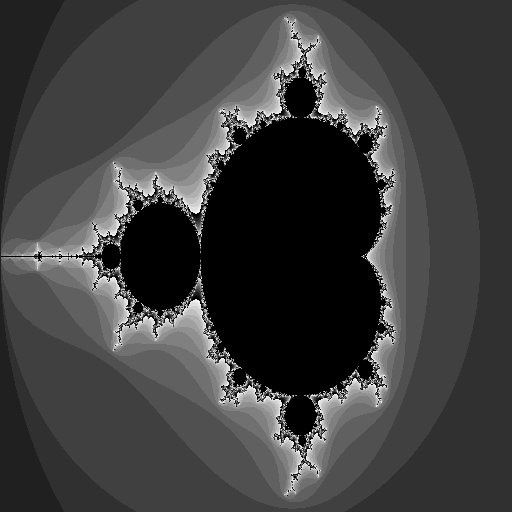
\includegraphics[width=.50\linewidth]{mandel}
%% 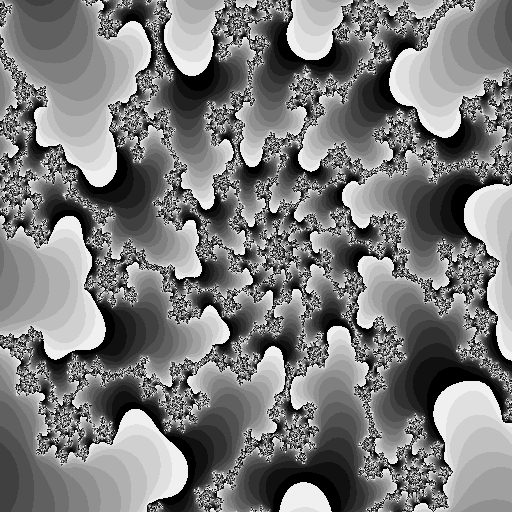
\includegraphics[width=.50\linewidth]{plate1}
%% \caption{ \emph{To the left:} Image of the Mandelbrot set with the parameters 
%% from table \ref{fig:mandeltable}. row ``mandel''.\newline
%% \emph{To the right:} A zoom in on the Mandelbrot image using the parameters 
%% from row ``mandel1''. }
%% \label{fig:mandel}
%% \end{figure}

%% \begin{figure} 
%% 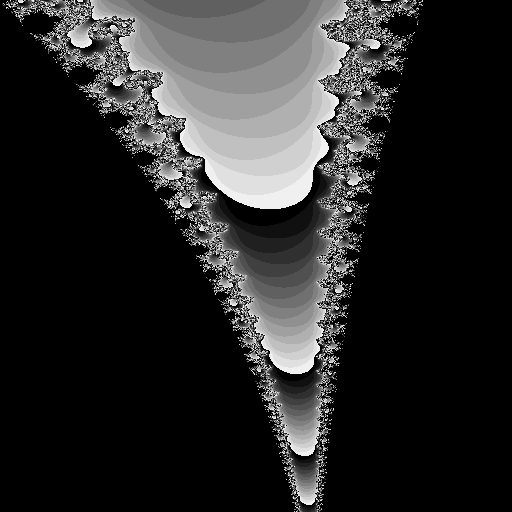
\includegraphics[width=.50\linewidth]{plate2}
%% 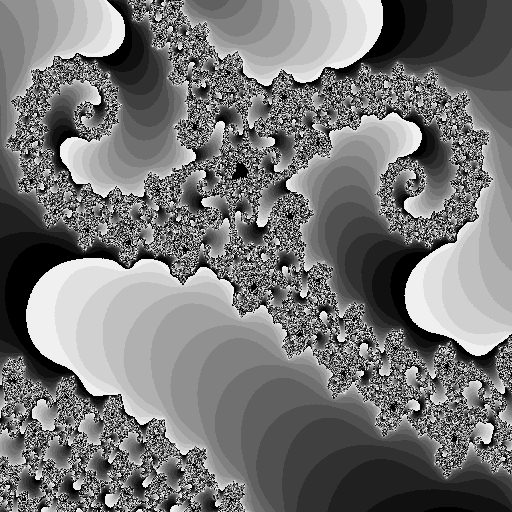
\includegraphics[width=.50\linewidth]{plate3}
%% \caption{\emph{To the left:} Mandelbrot image using parameters from row ``mandel2'' in fig. \ref{fig:mandeltable}. \newline
%% \emph{To the right:} Parameters from row ``mandel3''.}
%% \label{fig:mandel2}
%% \end{figure}

\begin{figure} 
\begin{small}
\begin{tabular}{| l | r | r | r | r | r | }
\hline 
  Image & xmax & xmin & ymax & ymin & ms \\ \hline 
  mandel & 1.2 & -2.0 & 1.2 & -1.2 & 2.65 \\ \hline
  mandel1 & -0.690906 & -0691060 & 0.387228 & 0.387103 & 1.78 \\ \hline
  mandel2 & -0.723005 & -0.793114 & 0.140974 & 0.037822 & 6.79 \\ \hline
  mandel3 & -0.745388 & -0.745464 & 0.113030 & 0.112967 & 5.7 \\ \hline
\end{tabular}
\caption{ Running times for the Mandelbrot program.
The parameters ({\tt xmax}, {\tt xmin}, {\tt ymax}, {\tt ymin}) correspond
to zooming in on different areas of the generated images.}
%This table contains the parameters used when generating the 
%images in figures \ref{fig:mandel} and \ref{fig:mandel2}. The last column 
%contains the time it took to generate the images in ms. The timing results 
%where obtained using an GT650m GPU. }
\label{fig:mandeltable} 
\end{small}

\end{figure} 

%% ------------------------------------------------------------------------
%% Reduction
%% ------------------------------------------------------------------------
\subsubsection{Reduction}  
\label{sec:redOpt}


% Figures that illustrate optimisation effort of Reduction kernels 

%% \newcommand{\arrayLength}[1]{%
%%   \setcounter{arraycard}{0}%
%%   \foreach \x in #1{%
%%     \stepcounter{arraycard}%
%%   }%
%%   \the\value{arraycard}%
%% }  

% smrow{x}{y}{data}{largest_index}{identifier}
\newcommand{\smRow}[5] { 
  
 %                                       (INSANE!) 
  \node [draw, fill=gray!30,anchor=west] (#50) at (#1,#2) {\pgfmathparse{#3[0]}\pgfmathresult};   
  
  \ifnum#4>0
    \foreach[count=\i] \j in {1,...,#4} {
      \pgfmathtruncatemacro{\n}{int(\i) - 1};
      \pgfmathtruncatemacro{\m}{int(\i)};
      \node [draw, fill=gray!30,right=0cm of #5\n,anchor=west] (#5\m) {\pgfmathparse{#3[\j]}\pgfmathresult};   % {\j};   
    } 
  \fi
}


% smRowTiny{x}{y}{data}{largest_index}{identifier} 
\newcommand{\smRowTiny}[5] { 
  
 %                                       
  \node [draw, fill=gray!30,anchor=west,inner sep=1pt] (#50) at (#1,#2) {\tiny\pgfmathparse{#3[0]}\pgfmathresult};   
  
  \ifnum#4>0
    \foreach[count=\i] \j in {1,...,#4} {
      \pgfmathtruncatemacro{\n}{int(\i) - 1};
      \pgfmathtruncatemacro{\m}{int(\i)};
      \node [draw, fill=gray!30,right=0cm of #5\n,anchor=west,inner sep=1pt] (#5\m) {\tiny\pgfmathparse{#3[\j]}\pgfmathresult};   % {\j};   
    } 
  \fi
}

\newcommand{\seqRed}[3] { 
 \tikzset{sstyle/.style={anchor=west,draw,shape=circle,fill,inner sep=1pt}};
 \tikzset{cstyle/.style={anchor=west,draw,shape=circle,inner sep=0pt}};
 %\tikzstyle{every node}=[anchor=west,draw,shape=circle,fill,inner sep=1pt]

 \node [sstyle](r1) at (0+ #1,#2) {};
 \node [sstyle,right=.5mm of r1] (r2) {};
 \node [sstyle,right=.5mm of r2] (r3) {};
 \node [sstyle,right=.5mm of r3] (r4) {};

 
 \path [draw] (r1) -- (r2) ;
 \path [draw] (r2) -- (r3) ;
 \path [draw] (r3) -- (r4) ;
 
 % connectors 

 %\tikzstyle{every node}=[anchor=west,draw,shape=circle,inner sep=0pt]

 \node [cstyle,above=.5mm of r1] (#3c1) {};
 \node [cstyle,above=.5mm of r2] (#3c2) {};
 \node [cstyle,above=.5mm of r3] (#3c3) {};
 \node [cstyle,above=.5mm of r4] (#3c4) {};

 \node [cstyle,below=.5mm of r4] (#3c5) {};

 % wires 

 \path [draw] (r1) -- (#3c1) ;
 \path [draw] (r2) -- (#3c2) ;
 \path [draw] (r3) -- (#3c3) ;
 \path [draw] (r4) -- (#3c4) ;
 \path [draw] (r4) -- (#3c5) ;


}



%\foreach[count=\i] \j in {1,1,1,1,1,1,1,1} { 
%  \pgfmathtruncatemacro{\n}{int(\i)};
%  \node[draw=black] (a\n) at (\i,-2) {\j};
%}



\begin{figure} 

% --------------------------------------------------------------------------- 
% Pair fmap 
% ---------------------------------------------------------------------------
\begin{minipage}{.45\linewidth} 
\begin{tikzpicture}[scale = 0.40]

\smRow{0}{0}{{0,1,2,3,4,5,6,7}}{7}{a}

\smRow{0}{-2}{{1,5,9,13}}{3}{b}

\smRow{0}{-4}{{6,22}}{1}{c}

\smRow{0}{-6}{{28,0}}{0}{d}  % HACK

%% \smRow{0}{0}{{0,1,2,3,4,5,6,7}}{7}{a}

%% \smRow{1.75}{-2}{{1,5,9,13}}{3}{b}

%% \smRow{2.5}{-4}{{6,22}}{1}{c}

%% \smRow{3}{-6}{{28,0}}{0}{d}  % HACK

% connections 


\path[->,draw=black] (a0.south) -- (b0.north) ; 
\path[->,draw=black] (a1.south) -- (b0.north) ; 

\path[->,draw=black] (a2.south) -- (b1.north) ; 
\path[->,draw=black] (a3.south) -- (b1.north) ; 

\path[->,draw=black] (a4.south) -- (b2.north) ; 
\path[->,draw=black] (a5.south) -- (b2.north) ; 

\path[->,draw=black] (a6.south) -- (b3.north) ; 
\path[->,draw=black] (a7.south) -- (b3.north) ; 


\path[->,draw=black] (b0.south) -- (c0.north) ; 
\path[->,draw=black] (b1.south) -- (c0.north) ; 

\path[->,draw=black] (b2.south) -- (c1.north) ; 
\path[->,draw=black] (b3.south) -- (c1.north) ; 

\path[->,draw=black] (c0.south) -- (d0.north) ; 
\path[->,draw=black] (c1.south) -- (d0.north) ; 


\end{tikzpicture} 

\end{minipage}
\hfill%hspace{2mm}%
% --------------------------------------------------------------------------- 
% Halve zip  
% ---------------------------------------------------------------------------
\begin{minipage}{.45\linewidth} 
\begin{tikzpicture}[scale = 0.40]

\smRow{0}{0}{{0,1,2,3,4,5,6,7}}{7}{a}

\smRow{0}{-2}{{4,6,8,10}}{3}{b}

\smRow{0}{-4}{{12,16}}{1}{c}

\smRow{0}{-6}{{28,0}}{0}{d}  % HACK

%% \smRow{0}{0}{{0,1,2,3,4,5,6,7}}{7}{a}

%% \smRow{1.75}{-2}{{4,6,8,10}}{3}{b}

%% \smRow{2.5}{-4}{{12,16}}{1}{c}

%% \smRow{3.25}{-6}{{28,0}}{0}{d}  % HACK

% connections 


\path[->,draw=black] (a0.south) -- (b0.north) ; 
\path[->,draw=black] (a4.south) -- (b0.north) ; 

\path[->,draw=black] (a1.south) -- (b1.north) ; 
\path[->,draw=black] (a5.south) -- (b1.north) ; 

\path[->,draw=black] (a2.south) -- (b2.north) ; 
\path[->,draw=black] (a6.south) -- (b2.north) ; 

\path[->,draw=black] (a3.south) -- (b3.north) ; 
\path[->,draw=black] (a7.south) -- (b3.north) ; 


\path[->,draw=black] (b0.south) -- (c0.north) ; 
\path[->,draw=black] (b2.south) -- (c0.north) ; 

\path[->,draw=black] (b1.south) -- (c1.north) ; 
\path[->,draw=black] (b3.south) -- (c1.north) ; 

\path[->,draw=black] (c0.south) -- (d0.north) ; 
\path[->,draw=black] (c1.south) -- (d0.north) ; 



\end{tikzpicture} 

\end{minipage}

%% \caption{\emph{Left:} {\tt evenOdds} - {\tt zipWith} reduction, leads to uncoalesced memory accesses.\newline
%% \emph{Right:} {\tt halve} - {\tt zipWith} reduction, leads to coalesced memory accesses.
%% This coalescing is most important during the very first phase, when data is 
%% read from global memory.} 

\label{fig:red1}
\end{figure} 



% ---------------------------------------------------------------------------
% Sequential reductions 
% ---------------------------------------------------------------------------


%% \begin{figure} 

%% \begin{tikzpicture}[scale = 0.40]

%% \smRowTiny{0}{{0,1,2,3,4,5,6,7,8,9,10,11,12,13,14,15,16,17,18,19,20,21,22,23,24,25,26,27,28,29,30,31}}{31}{a}

%% \seqRed{0}{-2}{redA}
%% \seqRed{2}{-2}{redB}
%% \seqRed{4}{-2}{redC}
%% \seqRed{6}{-2}{redD}
%% \seqRed{8}{-2}{redE}
%% \seqRed{10}{-2}{redF}
%% \seqRed{12}{-2}{redG}
%% \seqRed{14}{-2}{redH}

%% % connections 
%% \foreach[count=\i] \j in {redAc1,redAc2,redAc3,redAc4, 
%%                           redBc1,redBc2,redBc3,redBc4, 
%%                           redCc1,redCc2,redCc3,redCc4, 
%%                           redDc1,redDc2,redDc3,redDc4, 
%%                           redEc1,redEc2,redEc3,redEc4, 
%%                           redFc1,redFc2,redFc3,redFc4, 
%%                           redGc1,redGc2,redGc3,redGc4, 
%%                           redHc1,redHc2,redHc3,redHc4} {
%%   \pgfmathtruncatemacro{\n}{int(\i) - 1};
%%   \path[draw=black] (a\n.south) -- (\j.north) ; 
%% %\path[draw=black] (a1.south) -- (redAc2.north) ; 
%% %\path[draw=black] (a2.south) -- (redAc3.north) ; 
%% %\path[draw=black] (a3.south) -- (redAc4.north) ; 
%% } 

%% %next row of sM

%% \smRowTiny{-4}{{6,22,38,54,70,86,102,118}}{7}{b}

%% %connections 

%% \path[draw=black] (redAc5) -- (b0.north); 
%% \path[draw=black] (redBc5) -- (b1.north); 
%% \path[draw=black] (redCc5) -- (b2.north); 
%% \path[draw=black] (redDc5) -- (b3.north); 
%% \path[draw=black] (redEc5) -- (b4.north); 
%% \path[draw=black] (redFc5) -- (b5.north); 
%% \path[draw=black] (redGc5) -- (b6.north); 
%% \path[draw=black] (redHc5) -- (b7.north); 



%% %% \path[->,draw=black] (a0.south) -- (b0.north) ; 
%% %% \path[->,draw=black] (a1.south) -- (b0.north) ; 

%% %% \path[->,draw=black] (a2.south) -- (b1.north) ; 
%% %% \path[->,draw=black] (a3.south) -- (b1.north) ; 

%% %% \path[->,draw=black] (a4.south) -- (b2.north) ; 
%% %% \path[->,draw=black] (a5.south) -- (b2.north) ; 

%% %% \path[->,draw=black] (a6.south) -- (b3.north) ; 
%% %% \path[->,draw=black] (a7.south) -- (b3.north) ; 


%% %% \path[->,draw=black] (b0.south) -- (c0.north) ; 
%% %% \path[->,draw=black] (b1.south) -- (c0.north) ; 

%% %% \path[->,draw=black] (b2.south) -- (c1.north) ; 
%% %% \path[->,draw=black] (b3.south) -- (c1.north) ; 

%% %% \path[->,draw=black] (c0.south) -- (d0.north) ; 
%% %% \path[->,draw=black] (c1.south) -- (d0.north) ; 


%% \end{tikzpicture} 


%% \caption{Adding sequential reductions like this, reintroduces memory coalescing issues. 
%%  Consecutive threads nolonger access consecutive memory locations.} 

%% \label{fig:red1}
%% \end{figure} 




%% %%%%%%%%%%%%%%%%%%%%%%%%%%%%%%%%%%%%%%%%%%%%%%%%%%%%%%%%%%%%%%%%%%%%%%%%%%%
%%
%%  REINTRODUCE COALESCING
%%
%% %%%%%%%%%%%%%%%%%%%%%%%%%%%%%%%%%%%%%%%%%%%%%%%%%%%%%%%%%%%%%%%%%%%%%%%%%%%



\begin{figure} 

\begin{minipage}{0.45\linewidth}
\begin{tikzpicture}[scale = 0.40]

%\smRowTiny{0}{{0,1,2,3,4,5,6,7,8,9,10,11,12,13,14,15,16,17,18,19,20,21,22,23,24,25,26,27,28,29,30,31}}{31}{a}
\smRowTiny{0}{0}{{0,1,2,3,4,5,6,7,8,9,10,11,12,13,14,15}}{15}{a}

\seqRed{0}{-2}{redA}
\seqRed{2}{-2}{redB}
\seqRed{4}{-2}{redC}
\seqRed{6}{-2}{redD}
%\seqRed{8}{-2}{redE}
%\seqRed{10}{-2}{redF}
%\seqRed{12}{-2}{redG}
%\seqRed{14}{-2}{redH}

% connections 
\foreach[count=\i] \j in {redAc1,redAc2,redAc3,redAc4, 
                          redBc1,redBc2,redBc3,redBc4, 
                          redCc1,redCc2,redCc3,redCc4, 
                          redDc1,redDc2,redDc3,redDc4} {
                         
  \pgfmathtruncatemacro{\n}{int(\i) - 1};
  \path[draw=black] (a\n.south) -- (\j.north) ; 
} 

%next row of sM

%\smRowTiny{-4}{{6,22,38,54,70,86,102,118}}{7}{b}
\smRowTiny{0}{-4}{{6,22,38,54}}{3}{b}
%\smRowTiny{3}{-4}{{6,22,38,54}}{3}{b}


%connections 

\path[draw=black] (redAc5) -- (b0.north); 
\path[draw=black] (redBc5) -- (b1.north); 
\path[draw=black] (redCc5) -- (b2.north); 
\path[draw=black] (redDc5) -- (b3.north); 
%\path[draw=black] (redEc5) -- (b4.north); 
%\path[draw=black] (redFc5) -- (b5.north); 
%\path[draw=black] (redGc5) -- (b6.north); 
%\path[draw=black] (redHc5) -- (b7.north); 



%% \path[->,draw=black] (a0.south) -- (b0.north) ; 
%% \path[->,draw=black] (a1.south) -- (b0.north) ; 

%% \path[->,draw=black] (a2.south) -- (b1.north) ; 
%% \path[->,draw=black] (a3.south) -- (b1.north) ; 

%% \path[->,draw=black] (a4.south) -- (b2.north) ; 
%% \path[->,draw=black] (a5.south) -- (b2.north) ; 

%% \path[->,draw=black] (a6.south) -- (b3.north) ; 
%% \path[->,draw=black] (a7.south) -- (b3.north) ; 


%% \path[->,draw=black] (b0.south) -- (c0.north) ; 
%% \path[->,draw=black] (b1.south) -- (c0.north) ; 

%% \path[->,draw=black] (b2.south) -- (c1.north) ; 
%% \path[->,draw=black] (b3.south) -- (c1.north) ; 

%% \path[->,draw=black] (c0.south) -- (d0.north) ; 
%% \path[->,draw=black] (c1.south) -- (d0.north) ; 


\end{tikzpicture} 

%\label{fig:red1}

%\end{figure} 
\end{minipage}\hfill%\hspace{2mm}%
\begin{minipage}{0.45\linewidth}
%\begin{figure} 
%
\begin{tikzpicture}[scale = 0.40]

%\smRowTiny{0}{{0,1,2,3,4,5,6,7,8,9,10,11,12,13,14,15,16,17,18,19,20,21,22,23,24,25,26,27,28,29,30,31}}{31}{a}
\smRowTiny{0}{0}{{0,1,2,3,4,5,6,7,8,9,10,11,12,13,14,15}}{15}{a}

\seqRed{0}{-2}{redA}
\seqRed{2}{-2}{redB}
\seqRed{4}{-2}{redC}
\seqRed{6}{-2}{redD}
%\seqRed{8}{-2}{redE}
%\seqRed{10}{-2}{redF}
%\seqRed{12}{-2}{redG}
%\seqRed{14}{-2}{redH}

% connections 
\foreach[count=\i] \j in {redAc1,redBc1,redCc1,redDc1, 
                          redAc2,redBc2,redCc2,redDc2, 
                          redAc3,redBc3,redCc3,redDc3, 
                          redAc4,redBc4,redCc4,redDc4} {
                         
  \pgfmathtruncatemacro{\n}{int(\i) - 1};
  \path[draw=black] (a\n.south) -- (\j.north) ; 
} 

%next row of sM

%\smRowTiny{-4}{{6,22,38,54,70,86,102,118}}{7}{b}
%\smRowTiny{0}{-4}{{6,22,38,54}}{3}{b}
\smRowTiny{0}{-4}{{24,28,32,46}}{3}{b}
%\smRowTiny{3}{-4}{{6,22,38,54}}{3}{b}

%connections 

\path[draw=black] (redAc5) -- (b0.north); 
\path[draw=black] (redBc5) -- (b1.north); 
\path[draw=black] (redCc5) -- (b2.north); 
\path[draw=black] (redDc5) -- (b3.north); 
%\path[draw=black] (redEc5) -- (b4.north); 
%\path[draw=black] (redFc5) -- (b5.north); 
%\path[draw=black] (redGc5) -- (b6.north); 
%\path[draw=black] (redHc5) -- (b7.north); 



%% \path[->,draw=black] (a0.south) -- (b0.north) ; 
%% \path[->,draw=black] (a1.south) -- (b0.north) ; 

%% \path[->,draw=black] (a2.south) -- (b1.north) ; 
%% \path[->,draw=black] (a3.south) -- (b1.north) ; 

%% \path[->,draw=black] (a4.south) -- (b2.north) ; 
%% \path[->,draw=black] (a5.south) -- (b2.north) ; 

%% \path[->,draw=black] (a6.south) -- (b3.north) ; 
%% \path[->,draw=black] (a7.south) -- (b3.north) ; 


%% \path[->,draw=black] (b0.south) -- (c0.north) ; 
%% \path[->,draw=black] (b1.south) -- (c0.north) ; 

%% \path[->,draw=black] (b2.south) -- (c1.north) ; 
%% \path[->,draw=black] (b3.south) -- (c1.north) ; 

%% \path[->,draw=black] (c0.south) -- (d0.north) ; 
%% \path[->,draw=black] (c1.south) -- (d0.north) ; 


\end{tikzpicture} 
\end{minipage}

%% \caption{\emph{Left:} \textbf{BAD} Adding sequential reductions like this, reintroduces memory coalescing issues. Consecutive threads nolonger access consecutive memory locations.\newline
%% \emph{Right:} \textbf{GOOD} Using sequential reduction but maintaining coalescing} 

\label{fig:redSeq}
\end{figure} 


In this section, we implement a series of reduction kernels. The Obsidian 
reductions are implemented to take an associative operator as a parameter. 
In the benchmarking, the operation used will be addition and the elements 
will be $32$ bit integers. 

%\emph{ *** Probably good to say what type the elements of the arrays
%in the benchmarked CUDA has}

Some of the reduction 
kernels will also require that the operation is commutative. 
%A typical reduction is to sum up the elements of an array, here this is used 
%as the running example. In this section we implement a series of reduction 
%kernels. 
To illustrate the kind of low level control that an 
Obsidian programmer has over expressing details of a kernel, we show a series 
of reduction kernels, each with different optimisations applied. Many of the 
optimisations that are applied to the kernels are influenced by a 
tutorial presentation from NVIDIA~\citehl{reduction}.

%The figures \ref{fig:red1} and \ref{fig:redSeq} also illustrate various 
%tradeoffs that can be made while implemented reduction. 

%\emph{*** refer to fig:red1 and fig:redSeq in the right place.}

The kernels implemented in the following subsections use a variant of {\tt force}, 
called {\tt unsafeForce} that attempts to be clever about the insertion 
of synchronisation into the generated code. If the array that is being forced 
is shorter than the warp width, a synchronisation is not needed. It is called 
unsafe because when using push arrays there is still no absolute guarantee 
that the threads do not later write to indices that are used by threads that belong to another 
warp. Programmers should use {\tt unsafeForce} with care; it 
is however safe together with pull arrays. 

This section focuses on local reduction kernels. The construction of large 
reduction algorithms from these kernels will be illustrated in 
section~\ref{sec:Benchmarks}. 

\subsubsubsection{Reduction 1} 

Our first attempt at reduction combines adjacent elements repeatedly.
This approach is illustrated on the left of Figure \ref{fig:red1}. 
In Obsidian, this entails splitting the array into its even and its odd elements and using {\tt zipWith} to combine these. 
This procedure is then repeated until there is only one element left. This 
kernel will work for arrays whose length is a power of two. 

\begin{small} 
\begin{Verbatim}[samepage = true] 
red1 :: MemoryOps a
      => (a -> a -> a)
      -> SPull a
      -> BProgram (SPush Block a)
red1 f arr
  | len arr == 1 = return $ push arr
  | otherwise    = 
    do
      let (a1,a2) = evenOdds arr
      arr' <- unsafeForce $ zipWith f a1 a2
      red1 f arr'   
\end{Verbatim}
\end{small}

The above code describes what one block of threads does. To spread 
this computation out over many blocks and thus perform many simultaneous 
reductions, {\tt pConcatMap} is used (as before): 

\begin{small} 
\begin{Verbatim}[samepage = true] 
mapRed1 :: MemoryOps a 
              => (a -> a -> a) 
              -> DPull (SPull a) 
              -> DPush Grid a
mapRed1 f = pConcatMap $ pJoin . red1 f
\end{Verbatim}
\end{small} %$

This kernel does not perform well (as can be seen in Figure~\ref{fig:reducetable}). 
This may be attributed to the memory access pattern used. Remember that
one gets better performance on memory access when consecutive threads
access consecutive elements, which happens if
each thread accesses elements that are some stride apart. 

\subsubsubsection{Reduction 2}

{\tt red2} lets each thread access elements that are further apart. It does 
this by halving the input array and then using {\tt zipWith} on the halves (see Figure~ \ref{fig:red1}). 
This choice can only be made if the operator is commutative.  

\begin{small} 
\begin{Verbatim}[samepage = true] 
red2 :: MemoryOps a
           => (a -> a -> a)
           -> SPull a
           -> BProgram (SPush Block a)
red2 f arr
  | len arr == 1 = return $ push arr
  | otherwise    = 
    do
      let (a1,a2) = halve arr
      arr' <- unsafeForce $ zipWith f a1 a2
      red2 f arr'   
\end{Verbatim}
\end{small}

%This leads to the kind of access pattern that can be seen in the right half 
%of figure \ref{fig:red1}.

\subsubsubsection{Reduction 3} 

The two previous implementations of reduce write the final value into shared 
memory (as there is a {\tt force} 
in the very last stage). This means that the last element is stored into shared 
memory and then directly copied into global memory. This can be avoided by cutting 
the recursion off at length 2 instead of 1, and performing the last operation 
without issuing a {\tt force}. 

\begin{small} 
\begin{Verbatim}[samepage = true] 
red3 :: MemoryOps a
           => (a -> a -> a)
           -> SPull a
           -> BProgram (SPush Block a)
red3 f arr
  | len arr == 2 = 
      return $ 
      push $ 
      singleton $ f (arr ! 0) (arr ! 1) 
  | otherwise    = 
    do
      let (a1,a2) = halve arr
      arr' <- unsafeForce $ zipWith f a1 a2
      red3 f arr'
\end{Verbatim}
\end{small}


\subsubsubsection{Reduction 4} 

Now we have a set of three basic ways to implement reduction  and can start experimenting with adding 
sequential, per thread, computation. {\tt red4} uses
{\tt seqReduce}, which is provided by the Obsidian library and 
implements a sequential reduction that turns into a for loop in the generated 
CUDA code. The input array is split into 
chunks of 8 that are reduced sequentialy. The partial
results are reduced using the previously implemented ({\tt red3}). 

\begin{small}
\begin{Verbatim}[samepage = true] 
red4 :: MemoryOps a
           => (a -> a -> a)
           -> SPull a
           -> BProgram (SPush Block a)
red4 f arr =
  do
    arr' <- force $  
            pConcatMap (return . seqReduce f) 
                       (splitUp 8 arr)
    red3 f arr' 
\end{Verbatim}
\end{small}%$

As can be seen by the running times in Figure~\ref{fig:reducetable}, this optimisation 
did not come out well. The problem is that it reintroduces memory coalescing issues (see Figure \ref{fig:redSeq}). 

\subsubsubsection{Reduction 5} 

With {\tt red5}, the coalescing problem is dealt with by defining a new 
function to split up the array into sub arrays. The idea is that the 
elements in the inner arrays should be drawn from the original array in a strided fashion. 

\begin{small} 
\begin{Verbatim}[samepage = true] 
coalesce :: Word32 -> SPull a -> SPull (SPull a)
coalesce n arr =
  mkPull s $ \i ->
   mkPull n $ \j -> arr ! (i + fromIntegral s * j)
  where
    s = (len arr) `div` n 
\end{Verbatim}
\end{small}

\noindent
With {\tt coalesce} in place of {\tt splitUp}, {\tt red5} can be defined as: 

\begin{small} 
\begin{Verbatim}[samepage = true] 
red5 :: MemoryOps a
           => (a -> a -> a)
           -> SPull a
           -> BProgram (SPush Block a)
red5 f arr =
  do
    arr' <- force $  
            pConcatMap (return . seqReduce f)
                       (coalesce 8 arr)
    red3 f arr' 
  
\end{Verbatim}
\end{small}%$ 

\subsubsubsection{Reductions 6 and 7}

Lastly, we try to push the tradeoff between number of threads and sequential 
work per thread further. {\tt red6} and {\tt red7} represent  
changing {\tt red5} to reduce 16 and 32 elements in the sequential phase.
The performance of the fastest of these kernels is very satisfactory, at a level where the kernel is {\em memory bound}, that is constrained
by memory bandwidth.

\subsubsubsection{Larger local reductions} 
Figure \ref{fig:reducetablel} shows running time results for kernels that are 
very similar to the ones described above, but with a larger number 
of elements per local reduction (that is per block). This means that all the kernels need 
to introduce a small amount of sequentiality at the beginning. This is 
done by introducing a new force function:  

\begin{small}
\begin{Verbatim}[samepage=true] 
unsafeForce' arr | len arr > 1024 = return arr
                 | otherwise      = force  arr 
\end{Verbatim} 
\end{small}  

\noindent
{\tt unsafeForce'} exploits the fact that {\tt force} doesn't actually
change the elements of the array. 
Skipping the write into shared memory should still give the desired effect,
so replacing it with \verb!return! is safe. Two parallel phases are fused into one parallel phase that performs sequential work. 

This is a new way of introducing sequential work into kernels; unlike {\tt seqReduce}, it does not result in a for loop, but rather in an unrolled loop in the kernel.

%% \begin{small} 
%% \begin{Verbatim}[samepage = true] 

%% naiveReduceLocal :: MemoryOps a
%%                     => (a -> a -> a)
%%                     -> SPull a
%%                     -> BProgram (SPush Block a)
%% naiveReduceLocal f arr
%%   | len arr == 1 = return $ push Block arr
%%   | otherwise    = 
%%     do
%%       let (a1,a2) = halve arr
%%       arr' <- force $ zipWith f a1 a2
%%       naiveReduceLocal f arr'   
%% \end{Verbatim}
%% \end{small}

% --------------------------------------------------------------------------- 
% Measurements 
% ---------------------------------------------------------------------------
%% \begin{figure} 
%% \begin{small}
%% \begin{tabular}{| l | c | c | c | c | r | }
%% \hline 
%%   Kernel & Threads & Shared mem. & Sync opt. & Occupancy & ms \\ \hline 
%%   naive & 1024 & 16384 & N & 94.3  & 8.2 \\ \hline
%%   warp &  1024 & 16384 & Y & 94.4  & 8.2 \\ \hline
%%   seq1 & 512 & 4096 &  Y & 94.6   & 4.4 \\ \hline
%%   seq2 & 256 & 2048 & Y & 96.7 & 2.5 \\ \hline
%%   seq2b & 256 & 2048 & Y & 91.2  & 10.8 \\ \hline
%% \end{tabular}
%% \caption{ This table contains the execution time of a grid of 8192 reductions 
%% of each 2048 elements. The timing results where obtained using an GT650m GPU. }
%% \label{fig:reducetable} 
%% \end{small} 
%% \end{figure} 

\begin{figure} 
\begin{small}
\centering
\begin{tabular}{| l | c | c | c | c | r | }
\hline 
  Kernel & Threads & Shared mem. & ms & ms*\\ \hline 
  red1 & 1024 & 16384 & 9.619 & 1.678 \\ \hline
  red2 & 1024 & 16384 & 9.174 & 1.838 \\ \hline
  red3 & 1024 & 16384 & 8.795 & 1.855 \\ \hline
  red4 & 256 & 2048  & 10.839 & 2.120  \\ \hline
  red5 & 256 & 2048  & 2.608 &  0.445 \\ \hline
  red6 & 128 & 1024  & 2.471 &  0.442 \\ \hline
  red7 & 64 & 512  & 2.524 &    0.439 \\ \hline
\end{tabular}
\caption{ Execution time of a grid of 8192 reductions , each of
2048 elements on 
and on a GTX680 (ms*). The timing figures were obtained using the NVIDIA Profiler.}
\label{fig:reducetable} 
\end{small} 
\end{figure} 

\begin{figure} 
\begin{small}
\centering
\begin{tabular}{| l | c | c | c | c | r | }
\hline 
  Kernel & Threads & Shared mem. & ms & ms*\\ \hline 
  red1l & 1024 & 16384 & 8.883 & 1.762 \\ \hline
  red2l & 1024 & 16384 & 5.721 & 1.030  \\ \hline
  red3l & 1024 & 16384 & 5.377 & 0.980  \\ \hline
  red4l & 256 & 2048  & 11.202 & 2.201 \\ \hline
  red5l & 256 & 2048  & 2.476  & 0.440 \\ \hline
  red6l & 128 & 1024  & 2.471  & 0.442 \\ \hline
  red7l & 64 & 512  & 4.712    & 0.752\\ \hline
\end{tabular}
\caption{ Execution time of a grid of 4096 reductions, each of 4096 elements on a GT650m GPU (ms)
and on a GTX680 (ms*). The timing figures were obtained using the NVIDIA Profiler.}
\label{fig:reducetablel} 
\end{small} 
\end{figure} 





%% \begin{small} 
%% \begin{Verbatim}[samepage = true] 
%% reduceLocal :: MemoryOps a 
%%                => (a -> a -> a) 
%%                -> SPull a 
%%                -> BProgram (SPush Block a)
%% reduceLocal f arr | len arr == 2 = return $ push Block arr'
%%   where arr' = mkPullArray 1 $ \_ -> f (arr ! 0) (arr ! 1)
%% reduceLocal f arr | len arr < 32 =
%%   do
%%     let (a1,a2) = halve arr
%%     arr' <- write $ zipWith f a1 a2
%%     reduceLocal f arr'
%% reduceLocal f arr  = 
%%   do
%%     let (a1,a2) = halve arr
%%     arr' <- force $ zipWith f a1 a2
%%     reduceLocal f arr'   

%% \end{Verbatim}
%% \end{small}

%% \begin{small} 
%% \begin{Verbatim}[samepage = true] 
%% coalesce :: Word32 -> SPull a -> SPull (SPull a)
%% coalesce n (Pull m ixf) 
%%   = Pull (m `div` n) $ \i -> 
%%       Pull n $ \j -> ixf (i + (sizeConv (m `div` n)) * j)

%% reduce :: MemoryOps a 
%%           => (a -> a -> a) 
%%           -> SPull a 
%%           -> Program Block (SPush Block a)
%% reduce f arr =
%%   do
%%      arr' <- force $  mapT (return . seqReduce f) (coalesce 8 arr)
%%      reduceLocal f arr' 

%% reductions2 :: (ASize l, MemoryOps b)
%%                => (b -> b -> b)
%%                -> Pull l (SPull b)
%%                -> Push Grid l b
%% reductions2 f = mapG $ reduce f
%% \end{Verbatim}
%% \end{small}


%% \emph{*** Coalesced memory accesses}

%% \emph{*** Sequential computations}

%% \emph{*** Do not sync if inside a Warp} 


\subsubsection{Scan} 

Scan computes all the prefix sums of a sequence of values using 
a binary associative operator (and is familiar to Haskell
programmers as the {\tt scanl1} function).

Given an array of values $a_0,a_1,\ldots,a_n$ and associative operator $\oplus$,
the scan operation computes a new array: 

\begin{equation*} 
%\begin{array}{rcr} z & = & a \\ f(x,y,z) & = & x + y + z \end{array} 
  \begin{array} {rcl} 
    s_0 & = & a_0 \\
    s_1 & = & a_0 \oplus a_1 \\ 
    & \ldots & \\
    s_n & = & a_0 \oplus a_1 \oplus \ldots \oplus a_n
  \end{array}
\end{equation*} 


\begin{figure}
\begin{center}
\begin{tikzpicture} % [scale = 0.40]

% stage 1
\node [draw, fill=gray!30,anchor=west] (a0) {0};
\foreach[count=\i] \j in {1,2,3,4,5,6,7} {
  \pgfmathtruncatemacro{\n}{int(\i) - 1};
  \pgfmathtruncatemacro{\m}{int(\i)};
  \node [draw, fill=gray!30,right=21pt of a\n,anchor=west] (a\m) {\j};
}  

% stage 2

\foreach[count=\i] \j in {0,1,2,5,4,9,6,13} {
  \pgfmathtruncatemacro{\n}{int(\i) - 1};
  \node [draw, fill=gray!30,below=8pt of a\n] (b\n) {\j};
}  

%stage 3

\foreach[count=\i] \j in {0,1,3,6,4,9,15,22} {
  \pgfmathtruncatemacro{\n}{int(\i) - 1};
  \node [draw, fill=gray!30,below=8pt of b\n] (c\n) {\j};
}  


%stage 4

\foreach[count=\i] \j in {0,1,3,6,10,15,21,28} {
  \pgfmathtruncatemacro{\n}{int(\i) - 1};
  \node [draw, fill=gray!30,below=8pt of c\n] (d\n) {\j};
}  


%connections 

\path [draw] (a0.south) -- (b1.north);
\path [draw] (a1.south) -- (b1.north);

\path [draw] (a2.south) -- (b3.north);
\path [draw] (a3.south) -- (b3.north);

\path [draw] (a4.south) -- (b5.north);
\path [draw] (a5.south) -- (b5.north);

\path [draw] (a6.south) -- (b7.north);
\path [draw] (a7.south) -- (b7.north);

\path [draw] (a0.south) -- (b0.north);
\path [draw] (a2.south) -- (b2.north);
\path [draw] (a4.south) -- (b4.north);
\path [draw] (a6.south) -- (b6.north);

% -- 
\path [draw] (b1.south) -- (c2.north);
\path [draw] (b1.south) -- (c3.north);
\path [draw] (b0.south) -- (c0.north);
\path [draw] (b1.south) -- (c1.north);

\path [draw] (b2.south) -- (c2.north);
\path [draw] (b3.south) -- (c3.north);
\path [draw] (b6.south) -- (c6.north);
\path [draw] (b7.south) -- (c7.north);

\path [draw] (b5.south) -- (c6.north);
\path [draw] (b5.south) -- (c7.north);
\path [draw] (b4.south) -- (c4.north);
\path [draw] (b5.south) -- (c5.north);

% --
\path [draw] (c0.south) -- (d0.north);
\path [draw] (c1.south) -- (d1.north);
\path [draw] (c2.south) -- (d2.north);
\path [draw] (c3.south) -- (d3.north);
\path [draw] (c4.south) -- (d4.north);
\path [draw] (c5.south) -- (d5.north);
\path [draw] (c6.south) -- (d6.north);
\path [draw] (c7.south) -- (d7.north);

\path [draw] (c3.south) -- (d4.north);
\path [draw] (c3.south) -- (d5.north);
\path [draw] (c3.south) -- (d6.north);
\path [draw] (c3.south) -- (d7.north);



\end{tikzpicture} 
\end{center}
\caption{Sklansky parallel prefix network} 
\label{fig:Sklansky}
\end{figure}

%% ---------------------------------------------------------------------------
%% Seq Scan 
%% ---------------------------------------------------------------------------

\newcommand{\seqScan}[3] { 
 \tikzset{sstyle/.style={anchor=west,draw,shape=circle,fill,inner sep=1pt}};
 \tikzset{cstyle/.style={anchor=west,draw,shape=circle,inner sep=0pt}};
 %\tikzstyle{every node}=[anchor=west,draw,shape=circle,fill,inner sep=1pt]

 \node [sstyle](r1) at (0+ #1,#2) {};
 \node [sstyle,right=.5mm of r1] (r2) {};
 \node [sstyle,right=.5mm of r2] (r3) {};
 \node [sstyle,right=.5mm of r3] (r4) {};

 
 \path [draw] (r1) -- (r2) ;
 \path [draw] (r2) -- (r3) ;
 \path [draw] (r3) -- (r4) ;
 
 % connectors 

 %\tikzstyle{every node}=[anchor=west,draw,shape=circle,inner sep=0pt]

 \node [cstyle,above=.5mm of r1] (#3c1) {};
 \node [cstyle,above=.5mm of r2] (#3c2) {};
 \node [cstyle,above=.5mm of r3] (#3c3) {};
 \node [cstyle,above=.5mm of r4] (#3c4) {};

 \node [cstyle,below=.5mm of r1] (#3c5) {};
 \node [cstyle,below=.5mm of r2] (#3c6) {};
 \node [cstyle,below=.5mm of r3] (#3c7) {};
 \node [cstyle,below=.5mm of r4] (#3c8) {};


 % wires 

 \path [draw] (r1) -- (#3c1) ;
 \path [draw] (r2) -- (#3c2) ;
 \path [draw] (r3) -- (#3c3) ;
 \path [draw] (r4) -- (#3c4) ;
 
 \path [draw] (r1) -- (#3c5) ;
 \path [draw] (r2) -- (#3c6) ;
 \path [draw] (r3) -- (#3c7) ;
 \path [draw] (r4) -- (#3c8) ;


}



%Currently algorithms like scan pose a challenge to Obsidian.
Figure \ref{fig:Sklansky}
shows a standard divide and conquer decomposition of scan. Data
flows from top to bottom and boxes with two inputs are
operators. At each level, exactly half of the boxes are operators
and in an imperative language the algorithm would naturally be implemented
in-place.
%From this figure we can 
%read that half of the elements are altered in each parallel level of the algorithm 
%while the other half are untouched.
Since we cannot express in-place algorithms 
currently in Obsidian, this means that we need to copy unchanged values into a new array 
during each phase. The memory mapping gives us a ping-ponging implementation, but an in-place implementation would likely be faster.
%\emph{*** Too vague. Do we know??}

Also, the threads now do two different things 
(copy, or perform operation). 
One can have as many threads as elements, but then each must have
a conditional to decide whether to be a copy or operation thread.
%This can be implemented either by launching as many threads 
%as elements and performing a conditional in each thread to decide if this is a copy thread 
%or an operation thread. 
Or we can launch half as many threads and have each of them perform 
both a copy and an operation. 
We will show code for both of these options; the first is
easier to implement.
%We address these issues further in section \ref{sec:Future}, on future work. 


The Obsidian code below implements the scan network from Figure \ref{fig:Sklansky}, using as many threads as there are elements.
% and uses a 
%conditional to decide whether to copy or perform operations. 

\begin{small} 
\begin{Verbatim}[samepage=true]
sklansky :: (Choice a, MemoryOps a)
            => Int
            -> (a -> a -> a)
            -> SPull a
            -> BProgram (SPush Block a)
sklansky 0 op arr = return $ push arr
sklansky n op arr =
  do 
    let arr1 = binSplit (n-1) (fan op) arr
    arr2 <- force arr1
    sklansky (n-1) op arr2
\end{Verbatim} 
\end{small} % $

This is a kernel generator;
the (Haskell) {\tt Int} parameter can be used to generate kernels of various sizes by setting 
it to the log base two of the desired array size. 

The {\tt binSplit} combinator used in {\tt sklansky} is part of the Obsidian library 
and used to implement divide and conquer algorithms. It divides an array recursively in half 
a number of times (first parameter) and applies a computation to each part (second parameter). 
The operation applied in this case is {\tt fan}: 

\begin{small}
\begin{Verbatim}[samepage=true]
fan :: Choice a
       => (a -> a -> a)
       -> SPull a
       -> SPull a
fan op arr =  a1 `conc`  fmap (op c) a2 
    where 
      (a1,a2) = halve arr
      c = a1 ! fromIntegral (len a1 - 1)
\end{Verbatim}
\end{small}

It is the array concatenation ({\tt conc}) used in this function that introduces 
conditionals into the generated code. 

\subsubsubsection{Two elements per thread}


%Here, we try to optimise out implementation of Scan and also try to introduce 
%sequential work. By introducing sequential work per thread we can perform 
%larger instances of scan per GPU block. This is good since there is a maximum 
%number of threads in each block. 

%Obsidian provides the means to drop down to very low-level programming when 
%the higher level primitives do not operate as well as desired. The code listing 
%below illustrates this.

Both to avoid conditionals and to allow
for larger scans per block, we move to two elements per thread.
Each phase of the algorithm is a parallel for loop that is executed 
by half as many threads as there are elements to scan. The body of the loop
performs one operation and one copy, using bit-twiddling to compute indices.
Note the use of two {\em write functions} in sequence.
Similar patterns were used in our implementations of sorting networks~\citehl{Obsidian-Expressive}, for similar reasons.

%This code is a generator that given an integer that 
%refers to which parallel level of the algorithm we are interested in. It then 
%creates two separate parallel for loops; each running half as many threads as there 
%are elements. The first loop performs the operations between element and the 
%second just copies data. 

\begin{small} 
\begin{Verbatim}[samepage=true] 
phase :: Int 
         -> (a -> a -> a) 
         -> SPull a 
         -> SPush Block a
phase i f arr =
  Push l $ \wf -> ForAll sl2 $ \tid ->
  do
    let ix1 = insertZero i tid
        ix2 = flipBit i ix1
        ix3 = zeroBits i ix2 - 1
    wf (arr ! ix1) ix1
    wf (f (arr ! ix3) (arr ! ix2) ) ix2
  where
    l = len arr
    l2 = l `div` 2
    sl2 = sizeConv l2
\end{Verbatim} 
\end{small}

For an input of length $2^n$, $n$ phases
are composed as follows:

\begin{small} 
\begin{Verbatim}[samepage=true] 
sklansky2 :: MemoryOps a 
             => Int
             -> (a -> a -> a)
             -> SPull a
             -> BProgram (SPush Block a)
sklansky2 l f = compose [phase i f | i <- [0..(l-1)]]
\end{Verbatim}
\end{small} 

{\tt compose} takes a Haskell list of programs and composes 
them in sequence, forcing intermediate arrays between each step.
%Using Haskell for this kind of meta-programming is something that
%we plan to investigate further. 

\begin{small} 
\begin{Verbatim}[samepage=true] 
compose :: MemoryOps a
           => [SPull a -> SPush Block  a] 
           -> SPull  a
           -> BProgram (SPush Block  a)
compose [f] arr = return $ f arr
compose (f:fs) arr = 
  do
    let arr1 = f arr
    arr2 <- force arr1
    compose fs arr2
\end{Verbatim} 
\end{small} % $ 

Comparing the two kernels {\tt sklansky} and {\tt sklansky2} in the 
NVIDIA profiler indicates that {\tt sklansky2}, while being faster than 
{\tt sklansky} in many cases, has a worse memory loading behaviour. This 
indicates that tweaking the way data is loaded into shared memory may 
be beneficial in that kernel. 


\begin{small} 
\begin{Verbatim}[samepage=true] 
sklansky3 :: MemoryOps a
             => Int
             -> (a -> a -> a)
             -> SPull a
             -> BProgram (SPush Block a)
sklansky3 l f arr =
  do
    im <- force$ load 2 arr 
    compose [phase i f | i <- [0..(l-1)]] im 
\end{Verbatim}
\end{small}  % $

Here we use {\tt load 2} to realise loading of 2 elements per thread 
but in a strided way that is more likely to lead to a good memory access 
pattern. This function is an example of one of the custom ways to create a 
push array from a pull array mentioned in section \ref{sec:interplay}.
The results of these optimisations are shown in Figure~\ref{fig:scangraphs}.
To make a seriously fast local and global scan, we would need to add
more sequential work, as we did in the reductions. We do not yet know
if our inability to do in-place updates prevents us from competing with
hand-tuned CUDA scan code. 
%We hope to report more experiments in the final
%version of the paper.

%% Not shown here are the implementations of {\tt rv}, {\tt cv} and {\tt o}. 
%% {\tt rv} computes from a thread id one of the indices from which to read 
%% an element and perform operation on. {\tt o} provides the second element 
%% that also corresponds to the location of where to write the target element. 
%% {\tt cv} computes from the thread id an index that is supposed to be copied 
%% straight from the input array to the output array. The implementation 
%% of these functions are left out since they are highly specific to the 
%% algorithm. 

%% \begin{figure} 
%% \begin{small}
%% \centering
%% \begin{tabular}{| l | c | c | r | }
%% \hline 
%%   Kernel    & Threads & ms & ms*    \\ \hline 
%%   sklansky  & 1024    & x1 & x2     \\ \hline
%%   sklansky2 & 1024    & y1 & y2     \\ \hline

%% \end{tabular}
%% \caption{CAPTION CAPTION CAPTION}
%% \label{fig:scantable} 
%% \end{small} 
%% \end{figure} 
\begin{figure}
\begin{minipage}{.5\linewidth}
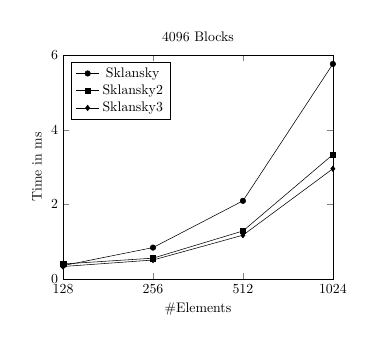
\begin{tikzpicture} [scale = 0.5]
\begin{axis} [xmax = 3, 
              xmin = 0, 
              ymax = 6,
              ymin = 0,
              % ytick = data,
              xtick = {0,1,2,3},
              xticklabels = {128,256,512,1024},
              legend entries = {Sklansky, Sklansky2, Sklansky3},
              legend pos = north west,
              xlabel = \#Elements, 
              ylabel = Time in ms,
              title = 4096 Blocks,
  ]         
  \addplot[color = black, 
           mark  = *,
           mark size = 2pt] coordinates {
    (0, 0.364 )
    (1, 0.847 )
    (2, 2.098 ) 
    (3, 5.762 )
  };
  \addplot[color = black, 
           mark  = square*,
           mark size = 2pt] coordinates {
    (0, 0.408 )
    (1, 0.564 )
    (2, 1.292 ) 
    (3, 3.336 )
  };
  \addplot[color = black, 
           mark  = diamond*,
           mark size = 2pt] coordinates {
    (0, 0.341 )
    (1, 0.514 )
    (2, 1.179 ) 
    (3, 2.957 )
  };
    


  
\end{axis}
\end{tikzpicture} 
\end{minipage}
\begin{minipage}{.5\linewidth}
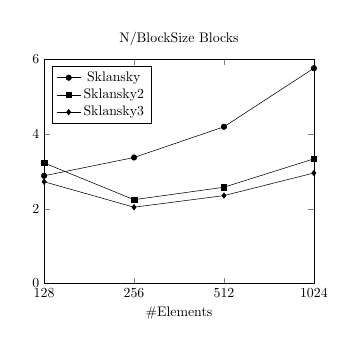
\begin{tikzpicture} [scale = 0.5]
\begin{axis} [xmax = 3, 
              xmin = 0, 
              ymax = 6,
              ymin = 0,
              % ytick = data,
              xtick = {0,1,2,3},
              xticklabels = {128,256,512,1024},
              legend entries = {Sklansky, Sklansky2, Sklansky3},
              legend pos = north west,
              xlabel = \#Elements,
              title = N/BlockSize Blocks
  ]         
  \addplot[color = black, 
           mark  = *,
           mark size = 2pt] coordinates {
    (0, 2.882 )
    (1, 3.372 )
    (2, 4.194 ) 
    (3, 5.762 )
  };
  \addplot[color = black, 
           mark  = square*,
           mark size = 2pt] coordinates {
    (0, 3.226 )
    (1, 2.242 )
    (2, 2.576 ) 
    (3, 3.336 )
  };
  \addplot[color = black, 
           mark  = diamond*,
           mark size = 2pt] coordinates {
    (0, 2.723 )
    (1, 2.041 )
    (2, 2.352 ) 
    (3, 2.957 )
  };
    


  
\end{axis}
\end{tikzpicture} 


\end{minipage}
\caption{\emph{left:}The time it takes to run 4096 blocks of varying sizes using our
different implementations of the Sklansky kernel. \newline
\emph{Right:} varies the number of blocks so that the number of elements is the 
same in each experiment. These results where obtained on an NVIDIA GT 650m using the 
NVIDIA Profiler.}
\label{fig:scangraphs}
\end{figure}

\subsection{Combining kernels to solve large problems} 
\label{sec:Benchmarks}

With Obsidian, we can experiment with details during the implementation 
of local computations. In section \ref{sec:CASESTUDIES}, we saw that the 
description of a local kernel involves its behavior when spread out 
over many blocks. However, solving large problems must sometimes make 
use of many different local kernels or the same local kernel used 
repeatedly. For now, we turn to CUDA for describing these algorithms. 
Here the procedure of making use of combinations of kernels is explained 
using large reduction as an example. 

\subsubsection{Large reductions}

We implement reduction of large arrays by running local kernels on blocks 
of the input array. If the local kernel reduces $ELT\_PER\_BLOCK$ elements to $1$ then 
this first step reduces $BLOCKS * ELT\_PER\_BLOCK$ elements into $BLOCKS$ partial results. 
The procedure is then repeated on the $BLOCKS$ elements until there is one 
value. 

Chosing {\tt red5l} from section \ref{sec:redOpt} and a block-size 
and local size of 4096 gives a 16 Million element reduction in only two stages. 

The CUDA code we need to write by hand is very simple and only describes the 
actual order of the kernels we wish to launch. We make no changes to the 
kernels themselves. The listing in figure~\ref{fig:cudareductioncode} shows an outline
of the CUDA code for launching {\tt red5l} to give $2^{24}$ (= 16777216)
element reduction.   

%% The listing in appendix \ref{app:A} shows an outline
%% of the CUDA code for launching {\tt red5l} to give $2^{24}$ (= 16777216)
%% element reduction.   
%% \pagebreak
\begin{figure} 
\begin{small}
\begin{Verbatim}[samepage=true] 

/* Define sizes to work on */ 
#define BLOCKS 4096
#define ELT_PER_BLOCK 4096
#define N (BLOCKS * ELT_PER_BLOCK)

int main(void) {
  
  /* Allocate host and device arrays */ 
  float *input, result; 
  float *dinput, *dresult; 
   
  input  = (float*)malloc(N*sizeof(float));
 
  cudaMalloc((void**)&dinput,N*sizeof(float));
  cudaMalloc((void**)&dresult,BLOCKS*sizeof(float));

  /* Generate input data */
  ... 

  /* Copy data to device */
  cudaMemcpy(dinput,
             input,
             N*sizeof(float),
             cudaMemcpyHostToDevice);

  
  /* Launch kernels */ 
  red5l<<<BLOCKS,256,512*sizeof(float)>>>(dinput,
                                             N,
                                             dresult);
  
  red5l<<<1,256,512*sizeof(float)>>>(dresult,
                                        4096,
                                        dresult); 

  /* Copy result from device */ 
  cudaMemcpy(&result,
             dresult,
             1*sizeof(float),
             cudaMemcpyDeviceToHost);

  
  /* Process data on host side, if needed */
  ... 

  return SUCCESS; 
\end{Verbatim} 
\end{small}
\caption{CUDA code that combines reduction kernels into reduction of a large array.}
\label{fig:cudareductioncode}
\end{figure}

This is just a very simple example of what CUDA code can look like. Part of 
the motivation for showing it is to make the presentation complete. 
We currently write this kind of CUDA skeleton by hand; section \ref{sec:Future} 
describes future work to improve this situation. 


\begin{figure}
\centering 
\begin{small}
\begin{tabular}{| l | r | r | r | }
\hline 
  System            & Elements & ms     & ms*   \\ \hline 
  Obsidian and CUDA & $2^{24}$  & 2.480  & 0.446 \\ \hline
  Accelerate        & $2^{24}$  & 2.716  & 0.478 \\ \hline
\end{tabular}
\caption{Running times of $2^{24}$ element reduction using Obsidian and CUDA 
or Accelerate. The results were obtained on a NVIDIA GT650m GPU (ms) 
and on a NVIDIA GTX680 GPU (ms*).}

\label{fig:CUDATABLE} 
\end{small}
\end{figure}

Table \ref{fig:CUDATABLE} shows the running time for the Obsidian together with 
CUDA $2^{24}$ element reduction compared to Data.Array.Accelerate. 
Again, the kernel generated from Obsidian is memory bound.
These values are 
interesting since they indicate that the Accelerate reduction skeleton is 
very well optimised, while maintaining generality. We expected this, since 
reduction corresponds directly to the Accelerate Fold skeleton, which
we believe to have been manually optimised as a one-time effort. It is also 
interesting that adding the second phase of reduction, in this case 
one instance of 4096 elements, only negligibly influences the running time.
%Remember that in section \ref{sec:redOpt}, {\tt red5l} runs in 2.5ms as well. 
%Choosing to round to one decimal place obscures any influence by that last phase. 


%\subsection{Scans} 
%\citehl{OLA} \citehl{LargeScan}


% ---------------------------------------------------------------------------
% RELATED WORK 
% --------------------------------------------------------------------------- 
\subsubsection{Related work}

There are many languages and libraries for GPU programming. Starting at the 
low-level end of the spectrum we have CUDA ~\citehl{CUDA}. CUDA is NVIDIA's 
name for the programming model and extended C language for their GPUs. 
It is 
the capabilities of CUDA that we seek to match with Obsidian,
while giving the programmer the benefits of having Haskell as a meta programming 
language. 
%% a high-level and 
%% functional programming language. 
%% \emph {*** Comment from Mary: I think this is not the right place to talk about
%% these limitations. Is it possible (nonetheless) to list what parts of
%% CUDA are (er) lifted to the Obsidian level? Just saying ``benefits of a high
%% level functional programming language seems too vague. We need to list them.]
%% }

%% There 
%% are low-level features of CUDA that we, as of yet, do not have control over 
%% from Obsidian. This is mainly related to in-\emph{warp} computations using 
%% registers and shuffle instructions to avoid using shared memory. A warp is a 
%% group of 32 threads (on current generation GPUs), that operate in a true SIMD 
%% fashion. In CUDA, being an imperative language with mutable arrays, in-place 
%% algorithms can also be easily expressed. Apart from these limitations it is 
%% the capabilities of CUDA that we seek to match with Obsidian,
%% while offering the programmer some of the benefits of a high-level and 
%% functional programming language. 

While remaining in the imperative world, but going all the way to the 
other end of the high-level - low-level spectrum, we have the NVIDIA
Thrust Library~\citehl{THRUST}.
Thrust offers a programming model where details of GPU architecture are 
completely abstracted away. Here, the programmer expresses algorithms 
using building blocks like: \emph{Sort}, \emph{Scan} and \emph{Reduce}.  

Data.Array.Accelerate is a language embedded in Haskell for GPU programming 
~\citehl{ACCELERATEDAMP11}. The abstraction level is comparable to that of Thrust. In 
other words, Accelerate hides most GPU details from the programmer. Accelerate 
provides a set of operations (that are parallel and suitable for GPU execution, 
much like in Thrust) implemented as skeletons. Recent work has permitted
the optimisation of Accelerate programs using fusion techniques to decrease
the number of kernel invocations needed (see reference ~\citehl{ACCOPT}).
%Accelerate programs are being optimised using using fusion 
%techniques to decrease the number of kernel invocations needed. 
It seems to us that when using Accelerate the programmer has no control over how to 
decompose his computation onto the GPU or how to make use of shared memory 
resources. For many users, remaining entirely within Haskell will be
a big attraction of Accelerate.     

Nikola ~\citehl{NIKOLA} is another language embedded in Haskell that occupies the 
same place as Accelerate and Thrust on the abstraction level spectrum. 

The systems above are all for flat data-parallelism, Bergstrom 
and Reppy are attempting nested data-parallelism by implementing a 
compiler for the NESL language for GPUs ~\citehl{NESL}. 

%\emph{*** Related work non-Haskell so as not to be too insular. Copperhead}

The Copperhead \citehl{copperhead} system compiles a subset of Python to run 
on GPUs. Much like other languages mentioned here, Copperhead identifies 
usages of certain parallel primitives that can be executed in parallel 
on the GPU (such as reduce, scan and map). But Copperhead also 
allows the expression of nested data-parallelism and is in that 
way different from both Accelerate and Obsidian.   

In reference ~\citehl{Finance}, Oancea et al. use manual transformations
to study a set of 
compiler optimisations for generating efficient GPU code from high-level 
and functional programs based on {\tt map}, {\tt reduce} and {\tt scan}. 
They tackle performance problems related to GPU programming, such as bad 
memory access patterns and diverging branches.
Obsidian enables easy exploration of decisions related to these issues.
%These are concepts that we try 
%to give the Obsidian programmer language support to reason about. 

In the implementation of Obsidian we use a very simple and direct approach 
to monad reification. Related to this work is the approach based on a 
continuation monad by Persson et al~\citehl{Generic}. Recent work by Sculthorpe et al. in reference ~\citehl{sculthorpe2013constrained} is also related. 
Our approach to monad reification is simpler but less general. 

% ---------------------------------------------------------------------------
% FUTURE WORK 
% --------------------------------------------------------------------------- 
\subsection{Future Work} 
\label{sec:Future}
%\emph{*** TEXT LEADING INTO THE THREE SUBSECTIONS} 

\subsubsection{Increase low level control} 

The capabilities of the GPU are changing and evolving. For example, it is now 
possible to do warp local computation that exchange values between threads 
using a set of {\tt shuffle} instructions. These kernels do not need to use 
shared memory to the same extent as the ones we generate. It would be interesting 
to try to incorporate these capabilities Obsidian. However, this 
would mean that plans to target both OpenCL and CUDA would have to be retired. 

In reference ~\citehl{CSORT}, we experiment with atomic operations 
and are forced to write our code in a very imperative style. The addition of mutable 
arrays and a set of operations on them could improve this situation 
while giving up purity. We will explore what the addition of mutable arrays to 
Obsidian would mean as future work. 

Being able to do in-place operations on arrays is beneficial to some algorithms. 
There are cases where in-place operation both simplifies implementation and improves performance.
Feldspar, an EDSL for Digital Signal Processing being developed in our group at Chalmers, has mutable arrays. In that case, it was Fast Fourier Transform
that pushed us towards this choice. Scan, in which elements must be copied
unchanged between arrays, while others are operated upon, may also push us towards mutable arrays. We need
to do more experiments before deciding whether or not to take this step,
particularly as we value the simpilicity of the current version of Obsidian.
%In 
%the case of scan, we need to copy many elements unchanged from one array to 
%another while performing operations on the other elements. We need a way to 
%implement in-place operations in Obsidian, maybe based on the mutable array 
%proposition above. 

\subsubsection{To automate or not to automate} 
Obsidian makes use of types that model the GPU hierarchy. This limits 
the kind of programs one can express but also ensures that what we can write 
is suitable for the GPU. An alternative is to remove these types and at the 
same time make the compiler more clever. This would move some of the 
required GPU detail knowledge from the programmer into compiler transformations. 
We have recently started a project to investigate this change of Obsidian
together with a Master's student. 

\subsubsection{To optimise or not to optimise} 
The version of Obsidian described here does not try to use any compiler optimisations techniques. Instead, we are expecting that the 
CUDA compiler will apply a good set of techniques, from common subexpression 
elimination to more GPU specific transformations. As future work, we 
will investigate to what extent this reliance on the CUDA
compiler is justified. Also, we want to 
see if there are high-level optimisations that we can perform more easily 
on our intermediate representations of GPU kernels than what is possible 
on low-level CUDA code. 

\subsubsection{Kernel Coordination} 

In section \ref{sec:Benchmarks}, we implemented large reduction using 
CUDA and kernels generated using Obsidian. This is something we want to 
be able to avoid. We envision a kernel coordination language embedded 
in Haskell where the programmer can express the kind of sequential 
and parallel compositions of kernels; note that this is different from 
composing two local computations into one, which we already have the 
capability to do. Having an embedded language for expressing full 
algorithms that make use of many different kernels would further 
improve the usability of Obsidian. We have started a project with the 
goal of implementing this language together with a Master's student. 

%\subsection{Exploiting Haskell, metaprogramming}
%We see opportunities for exploiting the fact that Obsidian is embedded
%in Haskell during kernel generation. Methods similar to the ``clever circuits'' techniques used in Lava may be interesting to explore. The use of search
%to find algorithmic decompositions that are well matched to the GPU is
%also an avenue that we would like to explore.

\subsection{What should the combinators be?}
In this latest version of Obsidian, we have at last got a system
that permits the construction of high performance kernels. But it is
clear that we need to think hard about the set of combinators that
we use to describe common patterns of parallel and sequential computation.
Our current choice is a bit ad hoc and needs to be generalised and made
more systematic. We will also explore the use of search to find algorithmic 
decompositions that are well matched to the GPU, exploiting the fact 
that Obsidian is embedded in a powerful host language.

% ---------------------------------------------------------------------------
% CONCLUSION
% --------------------------------------------------------------------------- 
\subsection{Conclusion}

%\emph{*** Come back to the contributions from the first page}

%\emph{*** Say something about how getting good performance
%out of machines with strange memory hierarchies is a
%general, important and pressing problem.}

Obsidian lends itself well to the kind of experimentation with low level 
GPU details that allow for the implementation of efficient kernels. This is 
illustrated in section \ref{sec:redOpt}, where we manage to apply techniques
used in the NVIDIA tutorial ~\citehl{reduction}. The case study also show hows we 
can compose kernels and thus reuse prior effort. 
%For example, {\tt red4} 
%to {\tt red7} all make use of {\tt red3} for their parallel phases. 

The use of GPU hierarchy generic functions makes the kernel code concise. The 
{\tt pMap} and {\tt pZipWith} functions are applicable both at block and grid 
level and are compiled into suitable parallel loops. The types that are used 
to model the GPU hierarchy also rule out any programs that we cannot 
very easily compile to the GPU. An alternative to this was discussed in 
the Future work section \ref{sec:Future}.


Our monad reification method certainly simplified
the implementation of Obsidian, and showed that the method works
well in practice (see reference ~\citehl{BB} for more details of the method).

While other approaches to GPU programming in higher level languages tend to deliberately abstract away from the details of the GPU, we persist in our aim of exposing architectural details of
the machine and giving the programmer fine control.
This is partly because trying to provide simple
but effective programming idioms is an interesting challenge.
More importantly, though, we are fascinated
by the problem of how to assist
programmers in making the subtle algorithmic decisions needed
to program
parallel machines with strange, programmer controlled
 memory hierarchies, and strange
constraints on memory access patterns. This problem is by no means
confined to GPUs, and it is both difficult and pressing.
We hope that Obsidian can form the basis for work in this area.

%We hinted at our simple and direct method of monad reification. This is described 
%in more detail in reference ~\citehl{BB}. 
%In Obsidian, we do not currently make 
%explicit use of the compositional nature of this method.   



% ---------------------------------------------------------------------------
% CONCLUSION 
% --------------------------------------------------------------------------- 
%\section{Conclusion}

% ---------------------------------------------------------------------------
% APPENDICES
% --------------------------------------------------------------------------- 
%\appendix
%\section{CUDA code}
%\label{app:A}



%This is the text of the appendix, if you need one.

% ---------------------------------------------------------------------------
% ACKNOWLEDGEMENTS
% --------------------------------------------------------------------------- 
\subsection*{Acknowledgments}
The work on monad reification presented in this paper is joint 
work between Josef Svenningsson and Joel Svensson. 

Push arrays were invented by Koen Claessen. The implementation 
of push arrays in Obsidian is targeted at 
GPUs and restricted compared to Koen's more general idea. Koen has 
also been a source of important insights and tips that have
improved this work greatly. 

This research has been funded by the Swedish Foundation for
Strategic Research (which funds the Resource Aware Functional 
Programming (RAW FP) Project) and by the
Swedish Research Council.



% We recommend abbrvnat bibliography style.

\bibliographystylehl{alpha}
\bibliographyhl{thesis}

% The bibliography should be embedded for final submission.

%\begin{thebibliography}{}
%\softraggedright

%\bibitem[Smith et~al.(2009)Smith, Jones]{smith02}
%P. Q. Smith, and X. Y. Jones. ...reference text...

%\end{thebibliography}

%\end{document}
